\documentclass[conference,10pt]{IEEEtran}
\IEEEoverridecommandlockouts
\usepackage[T1]{fontenc}
\usepackage{lmodern}
\usepackage{amsmath,amssymb}
\usepackage{booktabs}
\usepackage{array}
\usepackage{graphicx}
\usepackage{xcolor}
\usepackage{microtype}
\usepackage{url}
\usepackage[hidelinks]{hyperref}
\usepackage{balance}
\usepackage{siunitx}
\sisetup{detect-all}
\graphicspath{{figures/}}
\newcommand{\facil}{FACIL}
\newcommand{\pim}{PIM}
\newcommand{\MiB}{\,\mathrm{MiB}}
\newcommand{\KiB}{\,\mathrm{KiB}}

\title{FACIL Reproduction and Batch-Aware Decode Dispatch:\\
DRAM Re-layout and Analytical SoC--PIM Tradeoffs}
\author{\IEEEauthorblockN{Author 1 \quad and \quad Author 2}
\IEEEauthorblockA{Department of Computer Science and Engineering\\
Indian Institute of Technology Guwahati\\
\textit{Author names to be completed before submission}}
}
\begin{document}
\maketitle
\begin{abstract}
We reproduce the core memory-mapping argument of FACIL for Llama3-8B
FP16 linear weights using a standalone MapID model, a native modified
DRAMsim3 address decoder, and a controlled re-layout traffic proxy.
Four matrix classes pass placement, mixed-page-routing and matched-read
checks. Across 32 decoder blocks, serialized baseline read/write
completion brackets sum to 447.284 ms; adding an idealized SoC GEMM
roofline gives a projection-only prefill first-token proxy of
515.646--518.718 ms, compared with 68.362--71.434 ms for zero-copy
FACIL under identical ideal assumptions. Neither is measured TTFT.
Our original extension evaluates \emph{batch-width-aware decode-step
SoC/PIM dispatch} on FACIL's shared weight mapping. Under two explicitly
hypothetical PIM timing scenarios (5.325 and 20 ms/token), the modeled
SoC crossover for the main SoC efficiency setting occurs at batches
17 and 5, respectively. Dynamic traces and offline switching-cost
sensitivity show that switching can outperform the best static engine
without duplicating approximately 13.959 GB of linear weights; the
ideal duplication baseline matches its zero-overhead latency but
requires twice the weight storage. A 4-MiB DRAMsim3 diagnostic reports
66.2 GB/s for original-order reads and 201.65 GB/s for sequential reads,
with write results restricted to issue throughput. The DRAM traffic experiments and analytical execution models have
distinct scopes: attention, KV-cache traffic, PIM MAC timing, engine
transitions, and end-to-end decoding are not measured.
\end{abstract}

\begin{IEEEkeywords}
DRAM address mapping, processing-in-memory, LPDDR5, DRAMsim3,
LLM inference, batch-aware decode, execution dispatch, reproducibility.
\end{IEEEkeywords}

\section{Introduction}
On-device LLM inference uses the same weight matrices in distinct
computational regimes. During prefill, many input tokens are processed
with matrix--matrix multiplication (GEMM), favoring the SoC's GPU/NPU.
During autoregressive decode, matrix--vector multiplication (GEMV) is
memory-intensive and can benefit from bank-level PIM~\cite{facil}.
Near-bank PIM requires a specific distribution of weight chunks over
DRAM banks, whereas standard SoC software expects logically row-major
(or column-major) matrices. The on-demand re-layout baseline copies and
rearranges weights before SoC GEMM; \facil{} instead makes each huge
page's physical-to-DRAM address mapping selectable while preserving
conventional virtual addressing~\cite{facil}.

\textbf{Reproduction objective.} The reduced-scope assignment narrows the original
paper to a standalone mapping model, placement validation, DRAMsim3
re-layout-cost comparisons, and analytical PIM GEMV/TTFT estimates.
The study does not reproduce modified OS page tables, actual SoC measurements,
or a cycle-accurate PIM compute engine. The comparison is the
\emph{baseline with on-demand re-layout} versus the \emph{same
SoC--PIM architecture with \facil{}-style mapping and no extra
re-layout}. An additional implemented policy is evaluated separately.

\textbf{Questions.} (i) Can the paper's MapID selection and chunk
placement be reproduced? (ii) What DRAM traffic cost is associated
with the baseline's extra copy? (iii) What does eliminating that
cost imply for analytical TTFT, subject to explicit SoC/PIM model
assumptions? (iv) When can batch-width-aware dispatch improve
modeled decode linear-layer latency with a single weight copy?

\section{FACIL Mechanism and Comparison Boundary}
\subsection{Mapping and tensor placement}
\facil{} associates a mapping identifier (MapID) with a huge page.
The MapID selects which page-offset bits are interpreted as DRAM
row, bank, rank, channel, column and transfer-offset bits. In the
AiM-style mapping shown in Figs.~8--10 of~\cite{facil}, the low bits
keep each $(1,1024)$-element FP16 PIM chunk contiguous within a
\(2\KiB\) DRAM row. The PU-changing bits are placed above a
MapID-controlled number of DRAM-row bits. Multiple mapping choices
allow different matrix shapes to preserve PIM-operable placement.

Let \(n\) be the number of FP16 columns, \(b=2\) B/element,
\(K=1024\) elements/chunk, \(H=2\MiB\) the huge-page size, and
\(U=N_{\mathrm{ch}}N_{\mathrm{rank}}N_{\mathrm{bank}}\) the PIM-unit
count. The Fig.~9 selector is implemented using consistent byte units:
\begin{align}
R_{\mathrm{rounded}}&=2^{\lceil\log_2 n\rceil}b,\\
B_{\mathrm{perPU}}&=H/U,\\
\mathrm{MapID}&=\log_2\!\left(\frac{\min(R_{\mathrm{rounded}},B_{\mathrm{perPU}})}{Kb}\right),\label{eq:mapid}\\
\mathrm{partition}&=\bigl[R_{\mathrm{rounded}}>B_{\mathrm{perPU}}\bigr].\nonumber
\end{align}
This byte-normalized expression implements the intended bit-count
shown by the paper's examples; the printed pseudocode mixes
column-count and byte-size nomenclature. The independent mapping is reversible and is also integrated in the
native DRAMsim3 decoder and channel router for this reduced-scope test.

\subsection{Fair comparison boundary}
The on-demand baseline retains a PIM-operable weight representation
for decode and converts the matrix when the SoC needs its
conventional layout for prefill GEMM. \facil{} removes that
conversion by allowing the SoC to address the PIM-optimized
physical placement through normal virtual addresses. The original
paper's Fig.~5 motivates this comparison~\cite{facil}.

\begin{figure}[t]
\centering
\setlength{\fboxsep}{6pt}
\fbox{\begin{minipage}{0.91\columnwidth}
\small\centering
\textbf{On-demand baseline}\\[2pt]
PIM-formatted weights \(\longrightarrow\) \textbf{read + re-layout + write}
\(\longrightarrow\) SoC GEMM\\[5pt]
\rule{.85\linewidth}{.25pt}\\[4pt]
\textbf{\facil{}-style mapping}\\[2pt]
PIM-placed weights \(\longrightarrow\) \textbf{mapping-aware access}
\(\longrightarrow\) SoC GEMM\\[4pt]
\emph{Decode: PIM GEMV in both approaches}
\end{minipage}}
\caption{Comparison boundary. The absence of an extra \emph{re-layout}
operation is architectural; it is not a second DRAMsim3 timing
measurement. Computation and possible mapping-induced GEMM penalties
must be accounted for separately.}
\label{fig:comparison}
\end{figure}

\section{Implementation and Experimental Setup}
\subsection{Geometry and simulator}
The simulator uses four DRAMsim3 channels, two ranks/channel, 16 banks/rank,
2-MiB huge pages, and a $2\KiB$ AiM reference chunk consisting of
1,024 FP16 elements. The reference map decomposes a PIM chunk into
32-B DRAM transfers. Stock DRAMsim3 traces in this study instead issue
128-B transactions; each transaction groups four contiguous 32-B
reference transfers; the trace generator verifies that all four
map to the same channel/rank/bank/DRAM row with consecutive columns.

The \texttt{LPDDR5\_6400\_APPROX\_v1.ini} configuration uses
\texttt{rows=262144}, \texttt{columns=256} per device, four 64-bit
channels, two ranks/channel, 16 banks/rank, and \texttt{BL=16}.
The resulting \emph{aggregate} bank-row capacity is
$256\times64/8=2\KiB$. This is a synthetic row geometry chosen
for the AiM chunk model, not a validated physical LPDDR5 organization.

DRAMsim3 in this checkout implements an LPDDR4 command protocol, with
selected LPDDR5-6400-like timing parameters and
$t_{\mathrm{CK}}=0.3125\,\mathrm{ns}$. The ideal 256-bit aggregate
bandwidth at 6400 MT/s is 204.8 GB/s, \emph{not} an observed read
throughput and not proof of native LPDDR5 fidelity. The paper used a
separately modified DRAMsim-based PIM/LPDDR5 simulator~\cite{facil}.
Baseline re-layout source traces use verified physical-address encodings
for a conventional decoder. The \emph{native MapID-aware decoder and
channel router} were implemented and validated in the DRAMsim3
checkout, with a static per-huge-page registry supplied through
\texttt{FACIL\_PAGE\_MAP\_FILE}. This is software modeling, not
actual PTE-borne MapIDs, OS modification, or a PIM MAC engine.

\textbf{Trace-reader integrity.} A one-WRITE EOF regression test
produces exactly one WRITE and zero READs. Baseline stage counts are
checked against trace manifests and DRAMsim3 transaction statistics.

\subsection{Full-model linear-weight workload accounting}
The Llama3-8B configuration contains 32 decoder blocks; each block
uses two Q/O projections, two K/V projections, two FFN gate/up
matrices, and one FFN down matrix. The four distinct matrix shapes
listed in Table~\ref{tab:layers} therefore account for seven
linear weight matrices per block, totaling $416\MiB$ of FP16
weights per block. Across 32 blocks, the enumerated linear weights
occupy $13.0$ GiB, excluding embeddings, the output head,
normalization tensors and the attention cache. This is computed
from real model dimensions, not inferred from the small proxy runs.

A once-per-matrix read-plus-write traffic-only conversion would move
$26.0$ GiB for these linear weights. Even at the paper's Jetson
reference \emph{peak} external bandwidth of $204.8$ GB/s, this
requires at least $136.3$ ms of bus service if all these bytes
cross that interface, excluding all other work. This value is an
\emph{optimistic bandwidth floor}, not a measured baseline
re-layout latency and not TTFT. The aggregate may change if
weights are reused, transfers overlap, or actual software routes
differ. The included workload-accounting script calculates the matrix sizes
and transfer volume from tensor dimensions.

\subsection{Address-placement validation}
For every 1024-element FP16 chunk in four Llama3-8B matrix shapes,
DRAM-row and PU containment, boundary alignment,
and encode--decode round trips were verified. Row-wise
PU counts and crossings of 2-MiB page boundaries were also checked. Python unit
tests cover Figure 10 anchors, mapping invertibility and selected
per-page-ID behavior. A sampled numerical GEMV check computes
chunk-local partial sums and compares their reduction against
ordinary dot products. These are \emph{functional and placement}
tests, not bank lock-step execution tests.

\subsection{Native MapID decoder and channel routing prototype}
As an additional correctness gate, the existing
DRAMsim3 C++ \texttt{Config::AddressMapping()} was extended to optionally choose
an AiM-style bit mapping from a static MapID registry for each
2-MiB huge page. Crucially,
\texttt{BaseDRAMSystem::GetChannel()} was also changed to use the same decoded
channel; otherwise requests could be routed to a conventional
channel while the command scheduler decoded a different one.
Pages without registered MapIDs preserve conventional decoding.
The registry represents a reduced-scope test fixture, \emph{not}
modified OS page tables or a native PIM controller.

Independent Python/C++ validation checked 996 random/boundary
addresses and 2,162,688 non-aliasing 128-B blocks. A further 411
independent native decoder comparisons agreed, both MapID~2 and MapID~3
passed exhaustive single-page no-alias tests, and 16,384 accesses on
an unregistered page preserved conventional decoding. A 32-request routing test
showed conventional per-channel counts $(8,8,8,8)$ versus MapID~2
counts $(32,0,0,0)$. A 96-request mixed-page test produced
$(72,8,8,8)$ with zero writes. These tests establish decoder and
routing correctness, \emph{not} GEMM/PIM compute execution.

\subsection{Functional baseline re-layout verification}
Weight integrity was verified independently of the DRAMsim3 timing
engine. In the standalone software storage model, the PIM-oriented
physical representation is read through both an SoC logical-address
view and a PIM bank/row view; the on-demand baseline then reconstructs
the same logical weights into conventional contiguous storage.
Bytewise tests covered the four shapes in Table~\ref{tab:layers}, a
total of 2,162,688 distinct 128-B blocks; all compared equal.
Additional sample FP16 dot-product checks for K/V and FFN down passed.
These tests establish \emph{software-model data correctness}, not actual
memory-controller MapID support or PIM MAC execution.

\subsection{Baseline re-layout traffic experiment}
For the $2\KiB$-row configuration, each logical 128-B weight block
is read from its statically encoded PIM-oriented source and written
to a disjoint conventional row-major destination. Every
four underlying 32-B fragments, source uniqueness, destination
alignment, and channel counts are checked; for the K/V case this
means 262,144 32-B fragments and 65,536 distinct 128-B requests
per stage. DRAMsim3 replays \emph{transactions}, not the actual
CPU-side byte permutation.

The READ and WRITE stages run independently with the same
DRAMsim3 configuration and 256-cycle completion-search resolution. The reported sum
\begin{equation}
\widehat{T}_{\mathrm{re-layout}}=
\widehat{T}_{\mathrm{source\ read}}+
\widehat{T}_{\mathrm{destination\ write}}
\label{eq:copy}
\end{equation}
is a \emph{serialized sum of DRAM completion-time upper brackets}.
It is \emph{not} a rigorous bound on actual CPU/GPU conversion time:
CPU data rearrangement, caches, staged buffering and read/write
overlap are outside the simulator. The original paper similarly
excluded in-page reordering overhead from its DRAM-only
re-layout estimate~\cite{facil}. The absence of the extra copy
under \facil{} is a mechanism, not a second measured copy trace.

\begin{table}[t]
\caption{Target Llama3-8B FP16 matrices (geometry from the original paper's layer dimensions).}
\label{tab:layers}
\centering\footnotesize
\begin{tabular}{@{}lrrrl@{}}
\toprule
Layer class & Rows & Cols & Size & MapID \\
\midrule
Q/O & 4,096 & 4,096 & 32 MiB & 2 \\
K/V & 1,024 & 4,096 & 8 MiB & 2 \\
FFN gate/up & 14,336 & 4,096 & 112 MiB & 2 \\
FFN down & 4,096 & 14,336 & 112 MiB & 3 \\
\bottomrule
\end{tabular}
\end{table}

\section{Baseline Re-layout Evaluation}
\subsection{Baseline re-layout traffic and completion times}
\begin{table}[t]
\caption{Baseline DRAMsim3 serialized stage-completion upper
brackets under the 2-KiB aggregate bank-row configuration.
All values are in $\mu$s. These are read/write traffic proxies, not CPU
reordering or GPU compute times.}
\label{tab:copy}
\centering\footnotesize
\begin{tabular}{@{}lrrrr@{}}
\toprule
Matrix & Weight & Read & Write & Serial sum \\
 & (MiB) & ($\mu$s) & ($\mu$s) & ($\mu$s) \\
\midrule
Q/O & 32 & 736.000 & 165.920 & \textbf{901.920} \\
K/V & 8 & 184.560 & 41.120 & \textbf{225.680} \\
FFN gate/up & 112 & 2575.300 & 581.910 & \textbf{3157.210} \\
FFN down & 112 & 4826.080 & 581.910 & \textbf{5407.990} \\
\bottomrule
\end{tabular}
\end{table}

Four shape-specific traces were evaluated with
\texttt{measure\_relayout.py} and the 2-KiB bank-row configuration.
Every source READ and destination WRITE stage completed the expected
request count: 65,536 for K/V, 262,144 for Q/O, and 917,504 for
each FFN matrix. Each stage's completion is reported using an
upper bracket with 256-cycle resolution
($0.080\,\mu$s at $t_{\rm CK}=0.3125$ ns).

The FFN-down PIM-source READ bound is much larger than the equal-sized
FFN gate/up READ bound, reflecting different MapID placement and the
chosen trace-order memory behavior; this is not evidence of relative
GEMM or PIM compute speeds. The paper's 204.8-GB/s Jetson reference
is a \emph{theoretical aggregate peak}, not observed performance.

For 32 decoder blocks and per-block matrix multiplicities
(Q/O:2, K/V:2, gate/up:2, down:1), the \emph{sum} of these
independently measured stage upper brackets is
\begin{align}
\widehat T_{\rm copy,32}
&= 32\big[2(0.901920)+2(0.225680)\notag\\
&\qquad +2(3.157210)+5.407990\big]\notag\\
&=447.28352\,\mathrm{ms}.
\label{eq:copyfull}
\end{align}
This assumes every modeled weight matrix is converted once, all
reads/writes execute serially, and all stages retain the same
isolated DRAM conditions. It is \emph{not} a measured total LLM
re-layout, a bound on host-side byte permutation, or a measured TTFT.
The timing model uses trace manifests, independent READ/WRITE
transaction statistics, and the same configuration for each matrix
class. Only the DRAM traffic component is included in the reported
copy-stage sum.

\subsection{DRAM access-order bandwidth diagnostic}
For a 32,768-transaction (4-MiB) sample under the
same DRAMsim3 configuration, original-order READs complete within
63.36 $\mu$s (66.198 GB/s) while sequential-order READs complete
within 20.80 $\mu$s (201.649 GB/s), or 98.46\% of the configured
204.8 GB/s peak. This 3.05$\times$ read-throughput difference
supports access ordering as a major contributor to this \emph{sample}'s
baseline cost. Both WRITE runs report 20.80 $\mu$s, but their
completion criterion is \emph{commands issued}, not completed
writes. The result therefore does not establish completed-write
bandwidth or quantitatively explain the entire 447.284-ms
full-model copy-stage sum.
\begin{figure}[t]
\centering
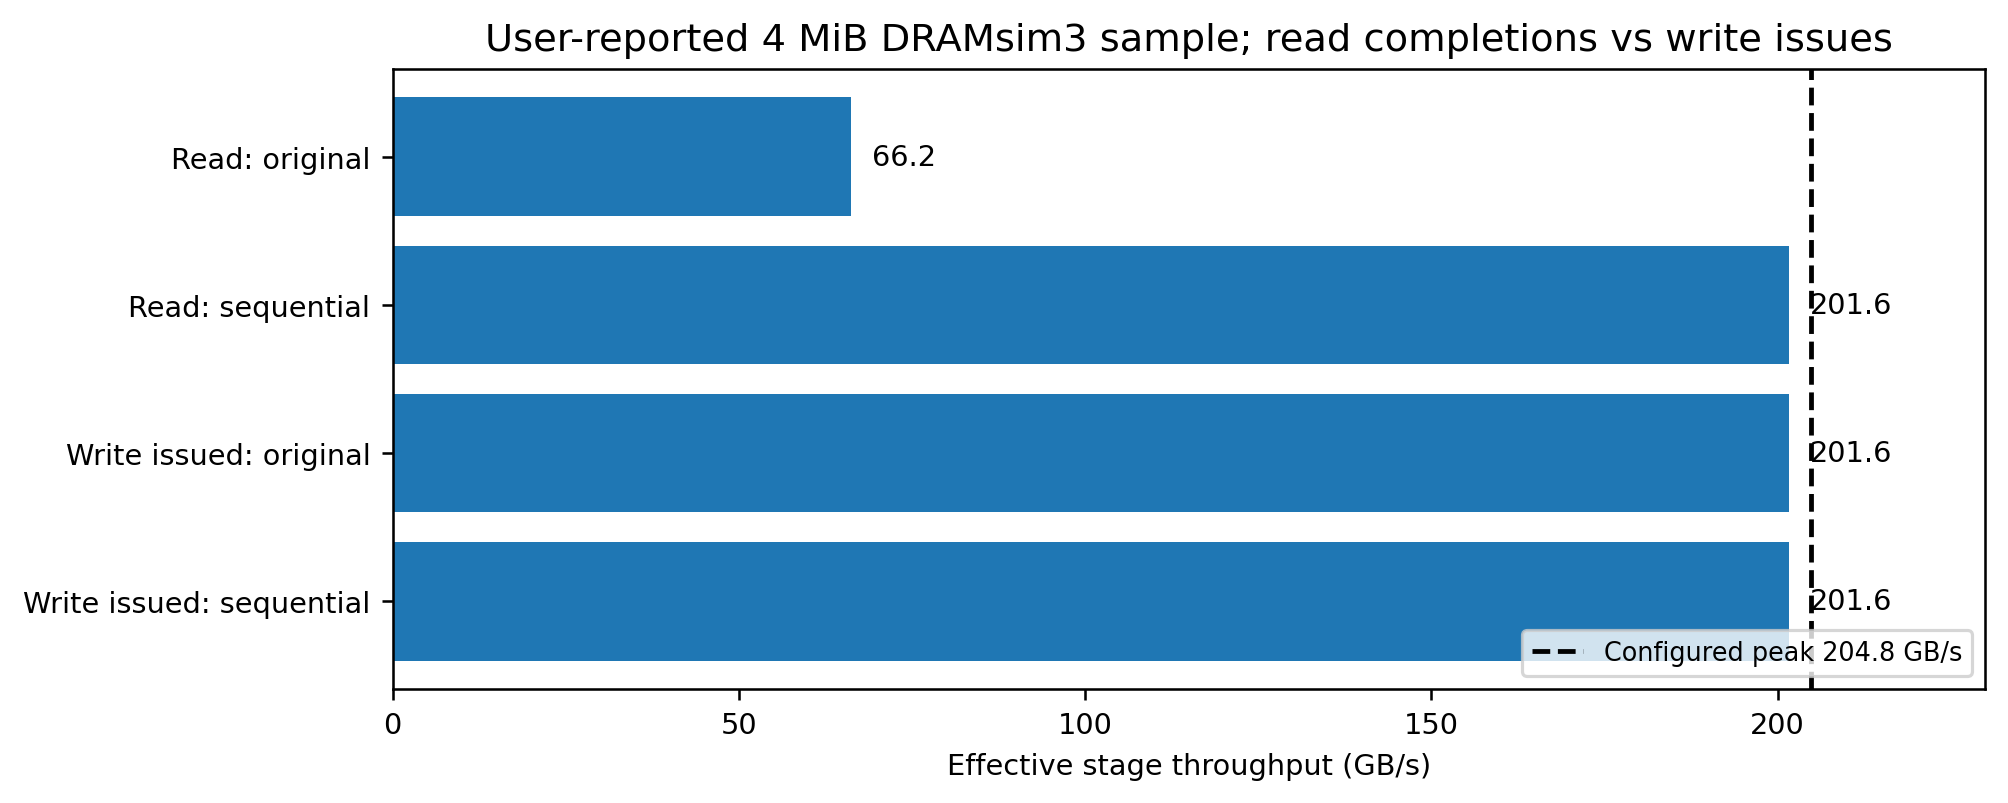
\includegraphics[width=\columnwidth]{exp5_sequential_bandwidth.png}
\caption{DRAMsim3 sample throughput. READ
rates use completed transactions; WRITE rates use issued commands
and must not be interpreted as completed-write bandwidth.}
\label{fig:exp5}
\end{figure}


\section{FACIL Mapping and Memory-Access Evaluation}
\subsection{FACIL MapID and chunk placement}
Under Fig.~10's two-channel example geometry, the reproduced
selector returns MapID 3 for \(2048\times8192\) and MapID 5 for
\(2048\times65536\), as in~\cite{facil}. Under the four-channel,
two-rank geometry, Table~\ref{tab:layers} gives the respective
values for the four actual Llama3-8B shapes. Across these shapes,
\(135{,}168\) chunks pass the implemented placement checks; 13
Python unit tests pass. The first three matrix shapes place each
logical row within one PU. For the \(4096\times14336\) compact
FFN-down shape, 2,048 rows use two PUs, 2,048 use three PUs,
and 48 rows cross huge-page boundaries. These findings reproduce
the selector and demonstrate reversible placement; they do
\emph{not} establish PIM lock-step timing.

\subsection{Native FACIL matched-read comparison}
The same sequence of useful FP16 weights was traced through the
conventional post-re-layout SoC view and the original PIM-placed
page(s) under native MapID decoding. All four categories pass
source/destination address-identity tests, all expected requests
complete, and no writes are emitted. The mapping differences in
Table~\ref{tab:matched} are \emph{DRAM read} differences, not GPU
GEMM slowdowns. The completion searches report upper brackets at
$0.3125$ ns DRAM cycles.
\begin{table}[t]
\caption{Matched sequential read completion upper brackets in
DRAMsim3 ($\mu$s); no extra copy in FACIL.}
\label{tab:matched}
\centering\footnotesize
\begin{tabular}{@{}lrrr@{}}
\toprule
Weight matrix & Reads & Conventional & FACIL MapID \\
\midrule
Q/O & 262,144 & 166.389 & 736.000 \\
K/V & 65,536 & 41.443 & 184.509 \\
FFN gate/up & 917,504 & 582.301 & 2575.300 \\
FFN down & 917,504 & 582.301 & 4826.080 \\
\bottomrule
\end{tabular}
\end{table}
\begin{figure}[t]
\centering
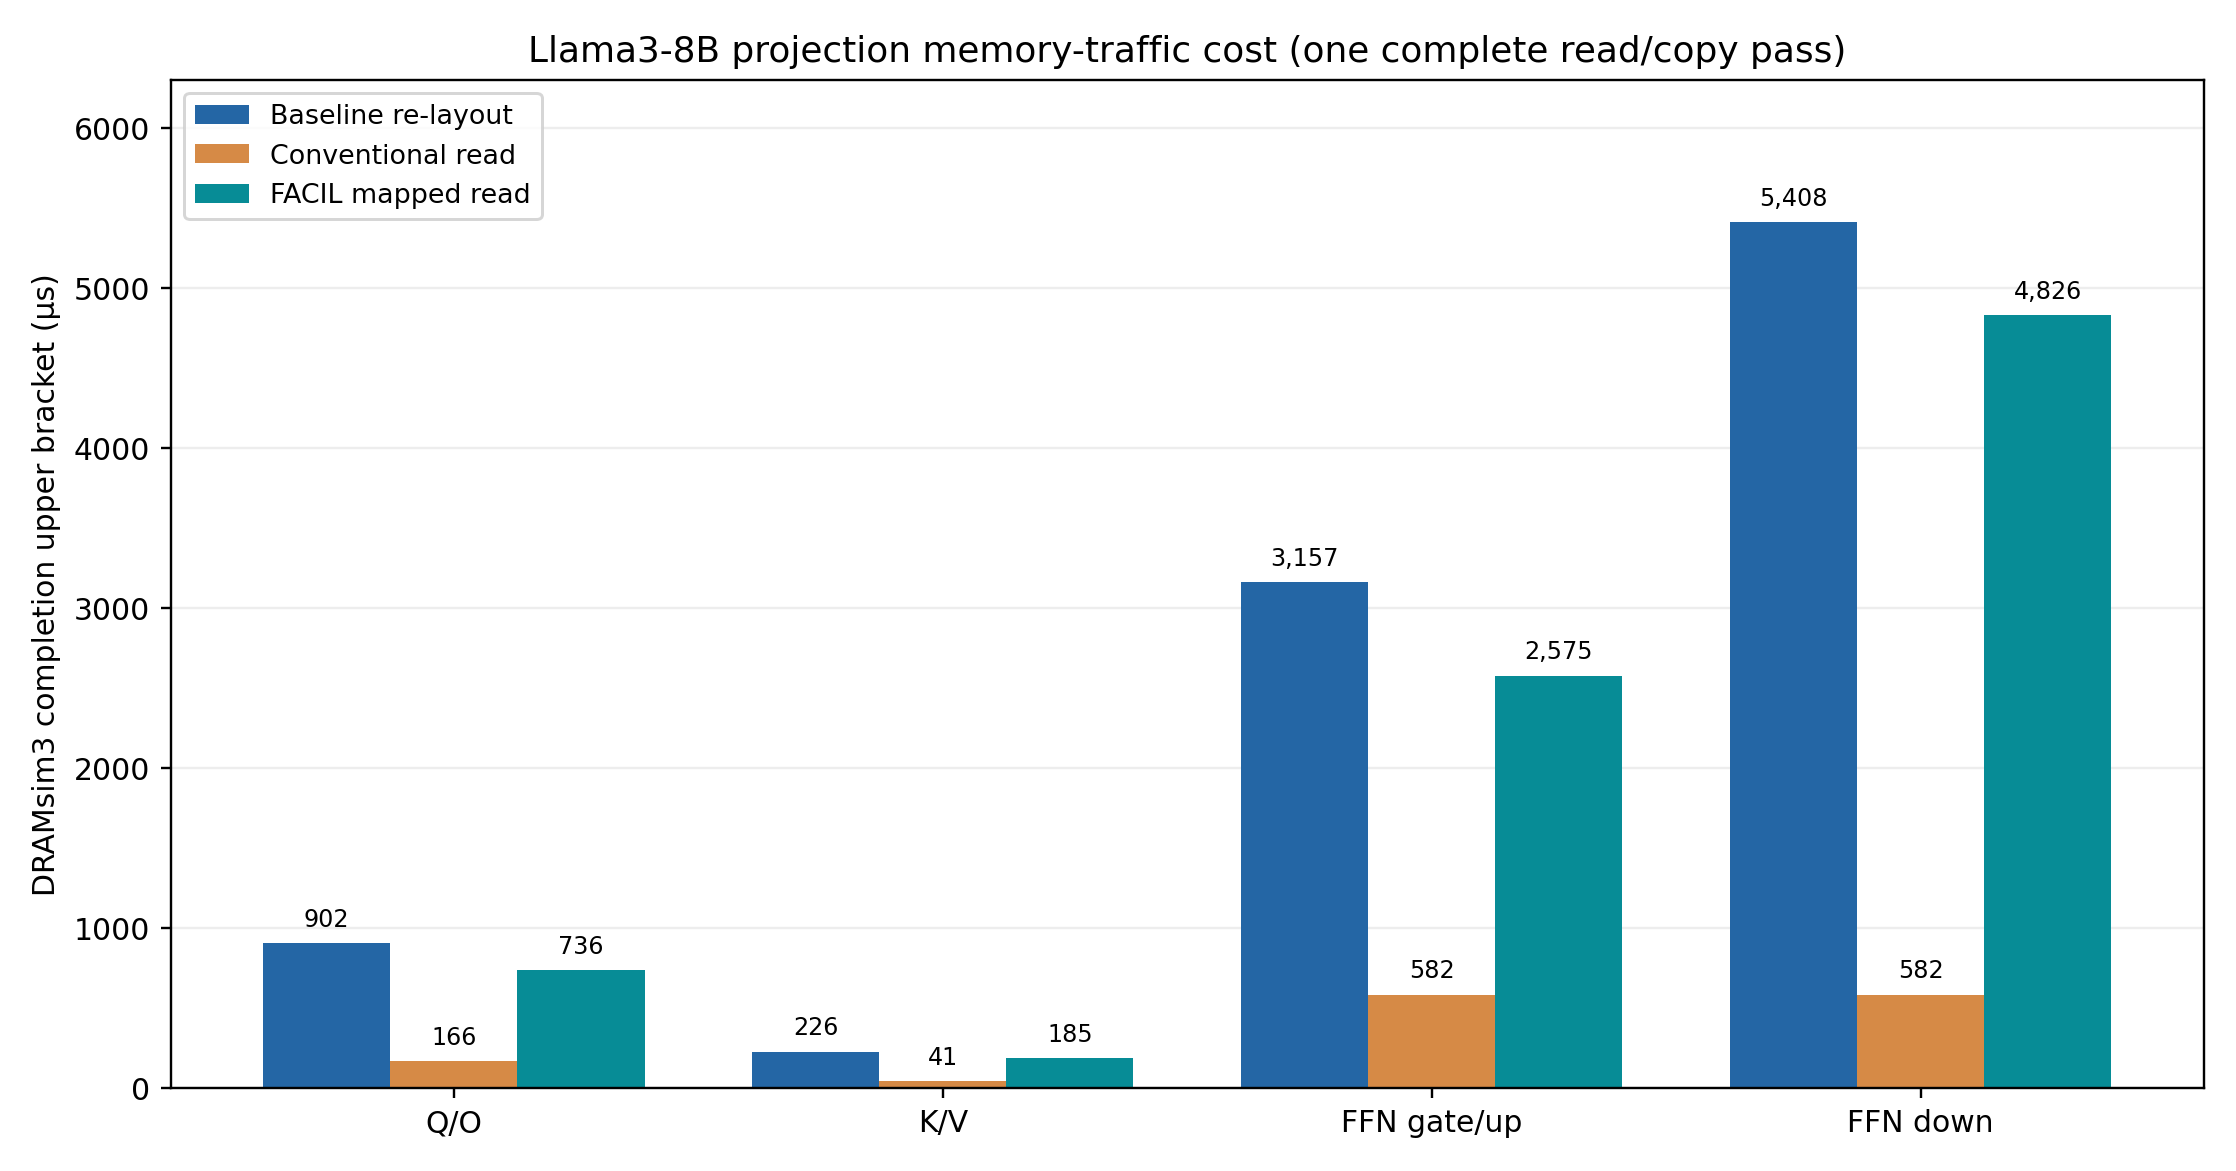
\includegraphics[width=\columnwidth]{read_vs_relayout.png}
\caption{Per-matrix DRAM traffic measurements: baseline extra-copy
upper brackets versus conventional and native FACIL matched reads.
These are distinct memory operations; displayed read times must not
be blindly added again to the roofline GEMM estimate.}
\label{fig:traffic}
\end{figure}

\section{Analytical First-Token Latency Models}
\subsection{SoC peak-roofline projection model}
For each FP16 linear projection with weights
$W\in\mathbb{R}^{M\times K}$ and $P$ prefill tokens, the model uses
$X\in\mathbb{R}^{K\times P}$ and
$Y=WX\in\mathbb{R}^{M\times P}$. Each GEMM requires
$F=2MKP$ floating-point operations under a two-FLOP
fused multiply-add convention. The modeled external traffic is
$B=2MK+2KP+2MP$ bytes: one FP16 read of all weights,
one input read, and one output write per independent GEMM.
Using FACIL Table~II's Jetson AGX Orin FP16 peak compute
(42.5 TFLOP/s) and theoretical bandwidth (204.8 GB/s),
\begin{align}
T_{\rm GEMM}^{\rm ideal} &= \max(T_{\rm calc},T_{\rm mem}),\notag\\
T_{\rm calc} &= \frac{2MKP}{42.5\times10^{12}},\notag\\
T_{\rm mem} &= \frac{2MK+2KP+2MP}{204.8\times10^9}.
\label{eq:gemm_analytical}
\end{align}
This ideal estimate is summed over all 224 independent linear
GEMMs in 32 decoder blocks; every projection is memory-bound
at the selected $P\le128$ under these assumptions.
\begin{table}[t]
\caption{Analytical SoC prefill \emph{linear projection} GEMM
peak-roofline estimates on Jetson (not measured GPU time,
not full TTFT).}
\label{tab:gemm}
\centering\footnotesize
\begin{tabular}{@{}rrrr@{}}
\toprule
$P$ & GEMMs & Wt. (GiB) & Time (ms) \\
\midrule
8 & 224 & 13.0 & 68.362 \\
16 & 224 & 13.0 & 68.567 \\
32 & 224 & 13.0 & 68.977 \\
64 & 224 & 13.0 & 69.796 \\
128 & 224 & 13.0 & 71.434 \\
\bottomrule
\end{tabular}
\end{table}
The accompanying dependency-free Python model self-checks
FLOPs, transfer bytes, tensor dimensions, 13-GiB weights,
224 linear GEMMs, and monotonicity across prefill lengths.
It excludes attention-score/value GEMMs, softmax, layer normalization,
nonlinearities, embeddings, output head, cache effects, kernel
launches, and resource contention. The peak-bandwidth assumption
is \emph{not} a measured DRAMsim3 bandwidth, and this is
neither a calibrated GPU model nor measured end-to-end prefill.
A GPU mapping slowdown cannot be established from this model alone.

\subsection{Baseline TTFT component proxy}
The baseline's \emph{projection-only component estimate} uses
(i) the 224 SoC FP16
linear-projection GEMMs modeled by the Jetson ideal peak roofline in
Table~\ref{tab:gemm} and (ii) the $447.283520$-ms sum of DRAMsim3
serialized re-layout stage-completion upper brackets in
Eq.~\eqref{eq:copyfull}:
\begin{equation}
\widehat T^{\mathrm{scope}}_{\mathrm{base,TTFT}}(P)
= T^{\mathrm{ideal}}_{\mathrm{SoC,linear}}(P)
 + \widehat T_{\mathrm{copy,32}}.
\label{eq:combined_base}
\end{equation}
\begin{table}[t]
\caption{Reduced-scope \emph{baseline TTFT component proxy}
for Llama3-8B (ms). This is not full or measured TTFT.}
\label{tab:combined_base}
\centering\footnotesize
\begin{tabular}{@{}rrrr@{}}
\toprule
Prefill $P$ & Ideal SoC GEMM & Copy stages & Proxy \\
\midrule
8 & 68.362 & 447.284 & \textbf{515.646} \\
16 & 68.567 & 447.284 & \textbf{515.851} \\
32 & 68.977 & 447.284 & \textbf{516.260} \\
64 & 69.796 & 447.284 & \textbf{517.079} \\
128 & 71.434 & 447.284 & \textbf{518.718} \\
\bottomrule
\end{tabular}
\end{table}
The table is calculated from full-precision component values before
rounding. This projection-only estimate is not the actual first-token
latency: attention-score/value operations, softmax, norms, nonlinearities,
embeddings/output head, sampling, GPU kernel/cache effects,
resource contention and possible overlap are excluded; host-side
byte permutation is also excluded as in the paper's DRAM-only
re-layout proxy. Furthermore, the SoC roofline assumes ideal
peak throughput, while the DRAM component is a sum of \emph{upper}
completion brackets. Therefore their sum is neither a rigorous
upper/lower TTFT bound nor an end-to-end TTFT measurement. The same explicitly truncated prefill boundary is applied to the
FACIL comparison, without pretending that omitted work is zero
in an actual LLM.

\subsection{Reduced-scope FACIL TTFT scenarios}
Let $G(P)$ be the same ideal 224-projection SoC GEMM model used in
Table~\ref{tab:combined_base}, and let $C=447.28352$ ms denote
serialized baseline re-layout stage brackets. Then
\begin{align}
\widehat{T}_{\rm base}(P)&=G(P)+C,\\
\widehat{T}_{\rm FACIL,ideal}(P)&=G(P),\\
\widehat{T}_{\rm FACIL,sens}(P)&=G(P)+D,\label{eq:facil_scenarios}
\end{align}
where the explicit \emph{mapping sensitivity} is
\begin{align}
D &= 32\sum_i n_i\!\left(T_{\rm FACIL,read,i}
 -T_{\rm conv,read,i}\right)\notag\\
  &= 308.96428\ \mathrm{ms}.
\end{align}
The multiplicities $n_i=(2,2,2,1)$ correspond to Q/O, K/V,
FFN gate/up, and FFN down. $D$ is obtained from whole-matrix
\emph{sequential-read} differences and hypothesizes one pass of
mapping-induced overhead per projection. Because the ideal GEMM
roofline already charges for weight traffic, only the \emph{increment}
is considered; even that transfer to GPU GEMM latency is \emph{not
experimentally established}. Thus the adjusted scenario is a
sensitivity analysis, \emph{not} a demonstrated FACIL GEMM slowdown.
\begin{table}[t]
\caption{Reduced-scope first-token \emph{component proxies}, ms.
None is measured end-to-end TTFT.}
\label{tab:facilttft}
\centering\scriptsize
\setlength{\tabcolsep}{3pt}
\begin{tabular}{@{}rrrrr@{}}
\toprule
$P$ & Baseline & Ideal & Sensitivity & Speedup \\
\midrule
8   & 515.646 & 68.362 & 377.327 & $1.367\times$ \\
16  & 515.851 & 68.567 & 377.531 & $1.366\times$ \\
32  & 516.260 & 68.977 & 377.941 & $1.366\times$ \\
64  & 517.079 & 69.796 & 378.760 & $1.365\times$ \\
128 & 518.718 & 71.434 & 380.399 & $1.364\times$ \\
\bottomrule
\end{tabular}
\end{table}
\begin{figure}[t]
\centering
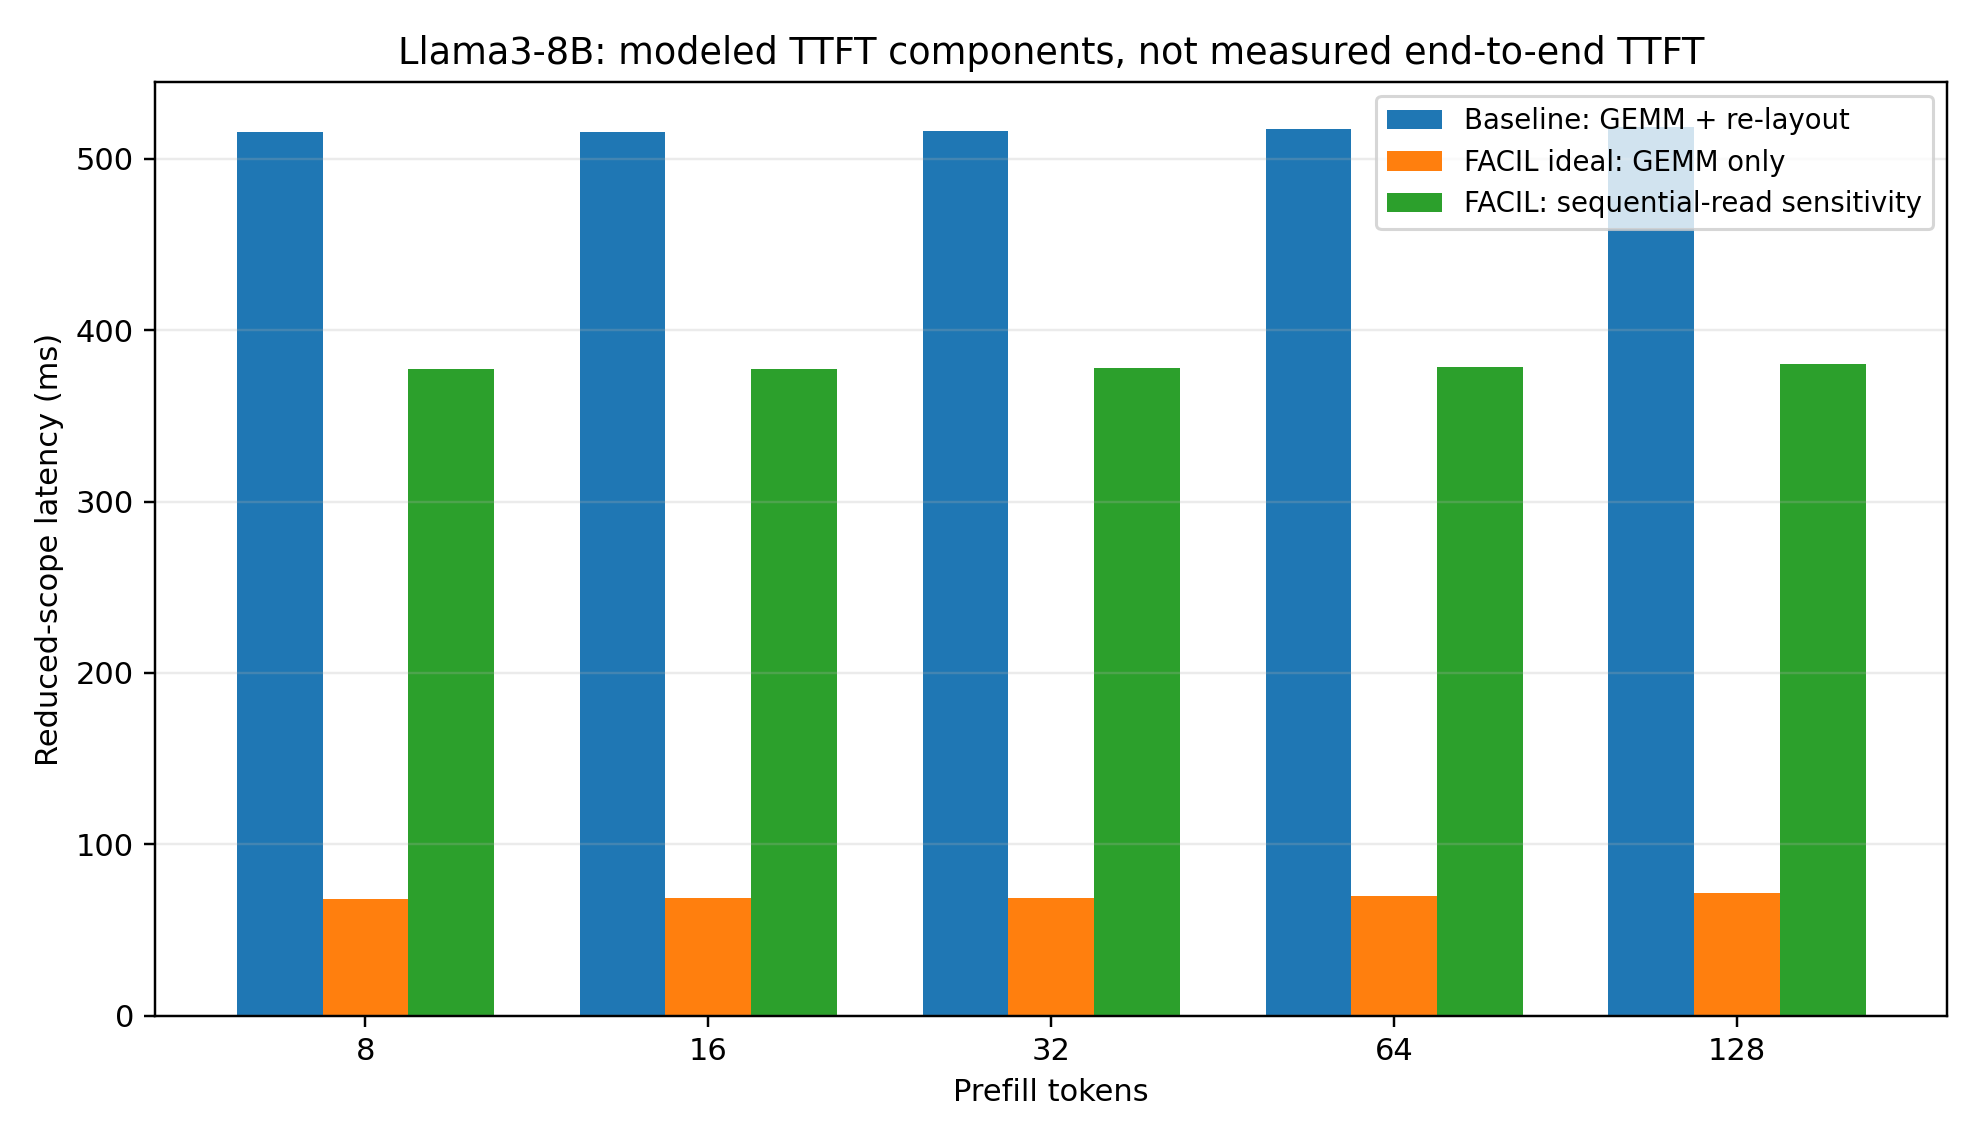
\includegraphics[width=\columnwidth]{ttft_comparison.png}
\caption{Baseline, ideal FACIL, and penalty-sensitive FACIL
first-token \emph{projection-only proxy}; common prefill operations
and actual GPU slowdown are not measured.}
\label{fig:ttftcomparison}
\end{figure}
\begin{figure}[t]
\centering
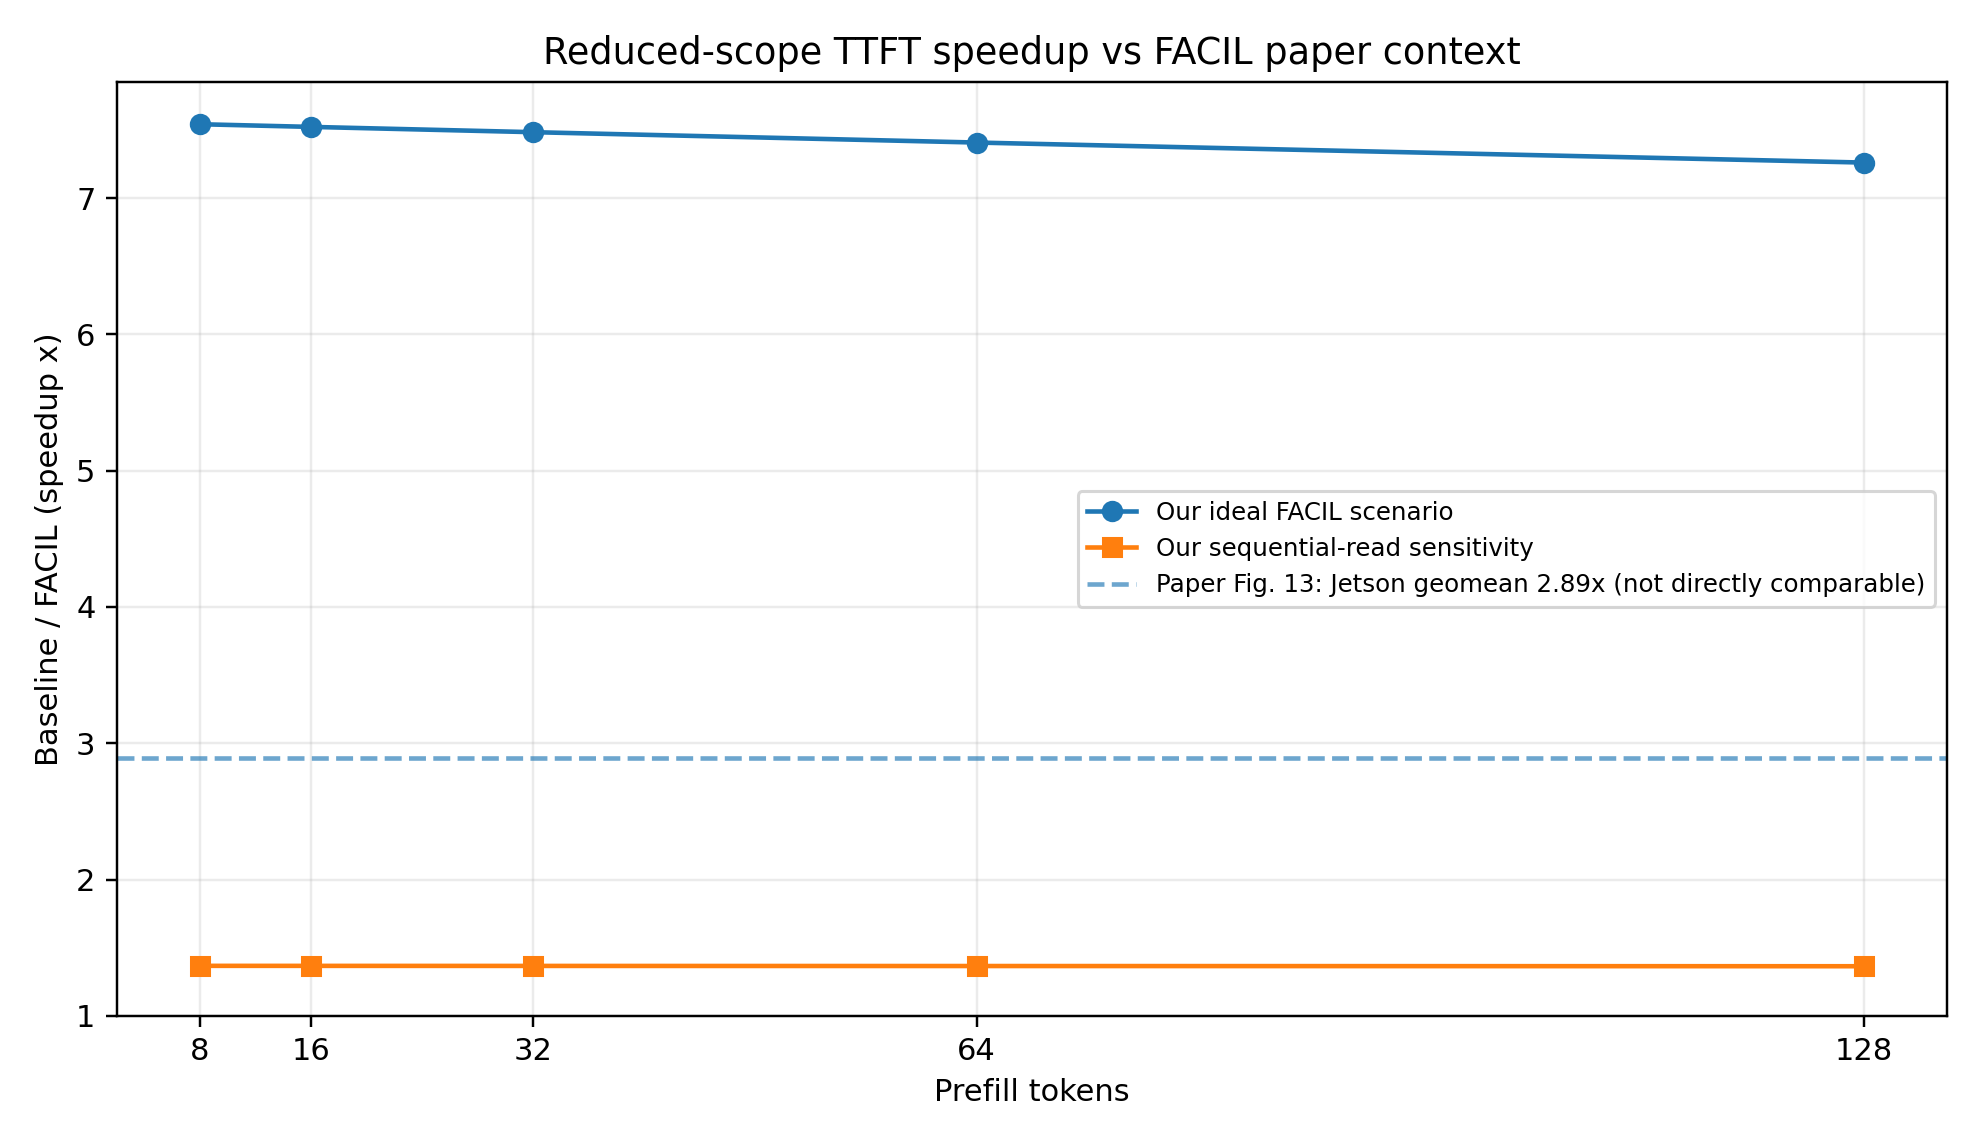
\includegraphics[width=\columnwidth]{ttft_speedups.png}
\caption{Model speedups compared with the published Jetson context
($2.89\times$ geometric mean in~\cite{facil}). The methodologies and
workload boundaries differ; the horizontal paper reference is not a
target that this proxy should numerically reproduce.}
\label{fig:speedups}
\end{figure}

\subsection{Analytical AiM-style GEMV and optional short prefill}
The assignment additionally requests an analytical PIM matrix--vector
model. For a weight matrix divided into $2$-KiB FP16 chunks, define
$W_i$ as the maximum number of chunks assigned to one processing bank
under validated MapID placement. The resulting counts are
$W_i=128,32,448,448$ for Q/O, K/V, FFN gate/up, and FFN down.
Under a \emph{hypothetical} effective PIM processing-wave latency
$\tau\in\{75,100,200\}$ ns, the optimistic GEMV formula is
\begin{equation}
\widehat{T}_{\rm PIM,GEMV,i}=W_i\tau,
\quad
\widehat{T}_{\rm PIM,prefill,i}(P)=P W_i\tau.
\label{eq:pimwave}
\end{equation}
For the seven projection categories repeated across 32 blocks,
this yields $3.9936$, $5.3248$, and $10.6496$ ms per generated
token at the three assumed wave times, respectively. These are
\emph{uncalibrated sensitivity inputs}, not published AiM timings
or measured DRAMsim3 PIM commands. The model does not charge for
input broadcasts, command issue/serialization, inter-bank or
cross-PU reductions, or other hardware scheduling. It especially
cannot prove efficient execution for FFN-down rows spanning multiple
PUs. Decode GEMV occurs after the first token and is therefore
\emph{not added} to ordinary prefill TTFT.

Following the paper's separate short-prefill scheduling idea
(its Fig.~15), the smaller modeled time is selected for
each prefill projection:
\begin{align}
\widehat{T}_{\rm dynamic}(P)
&=\sum_i 32n_i \min\bigl(S_i(P),P W_i\tau\bigr),\\
S_i(P)&=T_{\rm SoC,GEMM,i}(P)+\delta_i.
\end{align}
where $\delta_i=0$ for ideal SoC mapping and
$\delta_i=T_{\rm FACIL,read,i}-T_{\rm conv,read,i}$ in the
sequential-read sensitivity variant. For eight prompt tokens,
that sensitivity model produces $31.949$, $42.598$, and
$85.197$ ms at $75$, $100$, and $200$ ns/wave, respectively.
This is an \emph{additional conditional scenario}, not the measured
prefill policy or a replacement for Table~\ref{tab:facilttft}.
\begin{figure}[t]
\centering
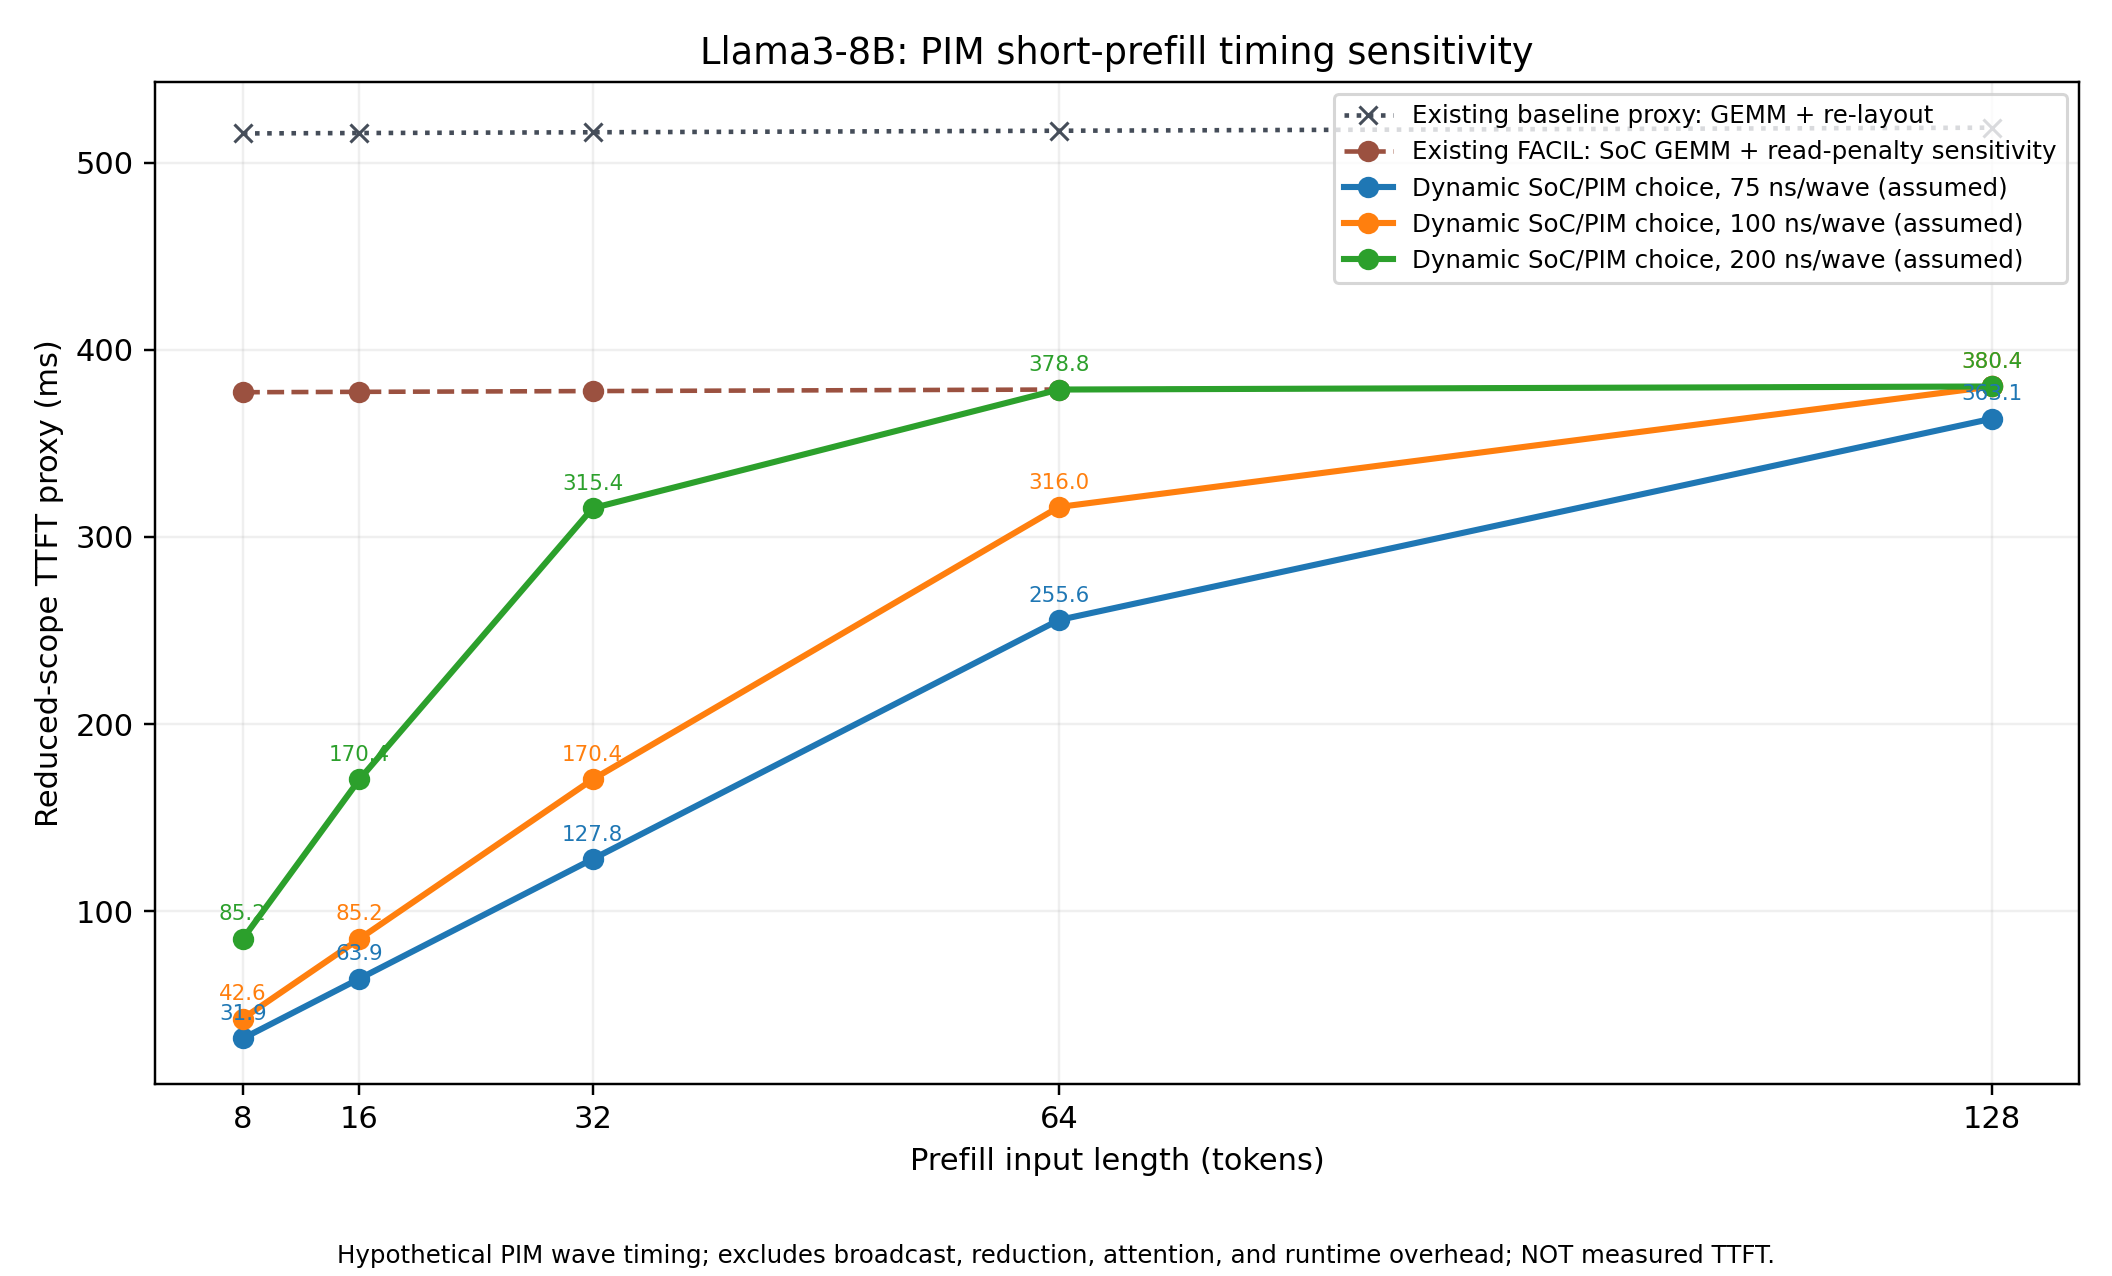
\includegraphics[width=\columnwidth]{pim_prefill_sensitivity.png}
\caption{Optional dynamic SoC/PIM prefill timing sensitivity at
hypothetical PIM wave latencies. Values are optimistic component
estimates; they exclude PIM staging/reduction overhead and are not
observed end-to-end TTFT.}
\label{fig:pimshort}
\end{figure}
\begin{figure}[t]
\centering
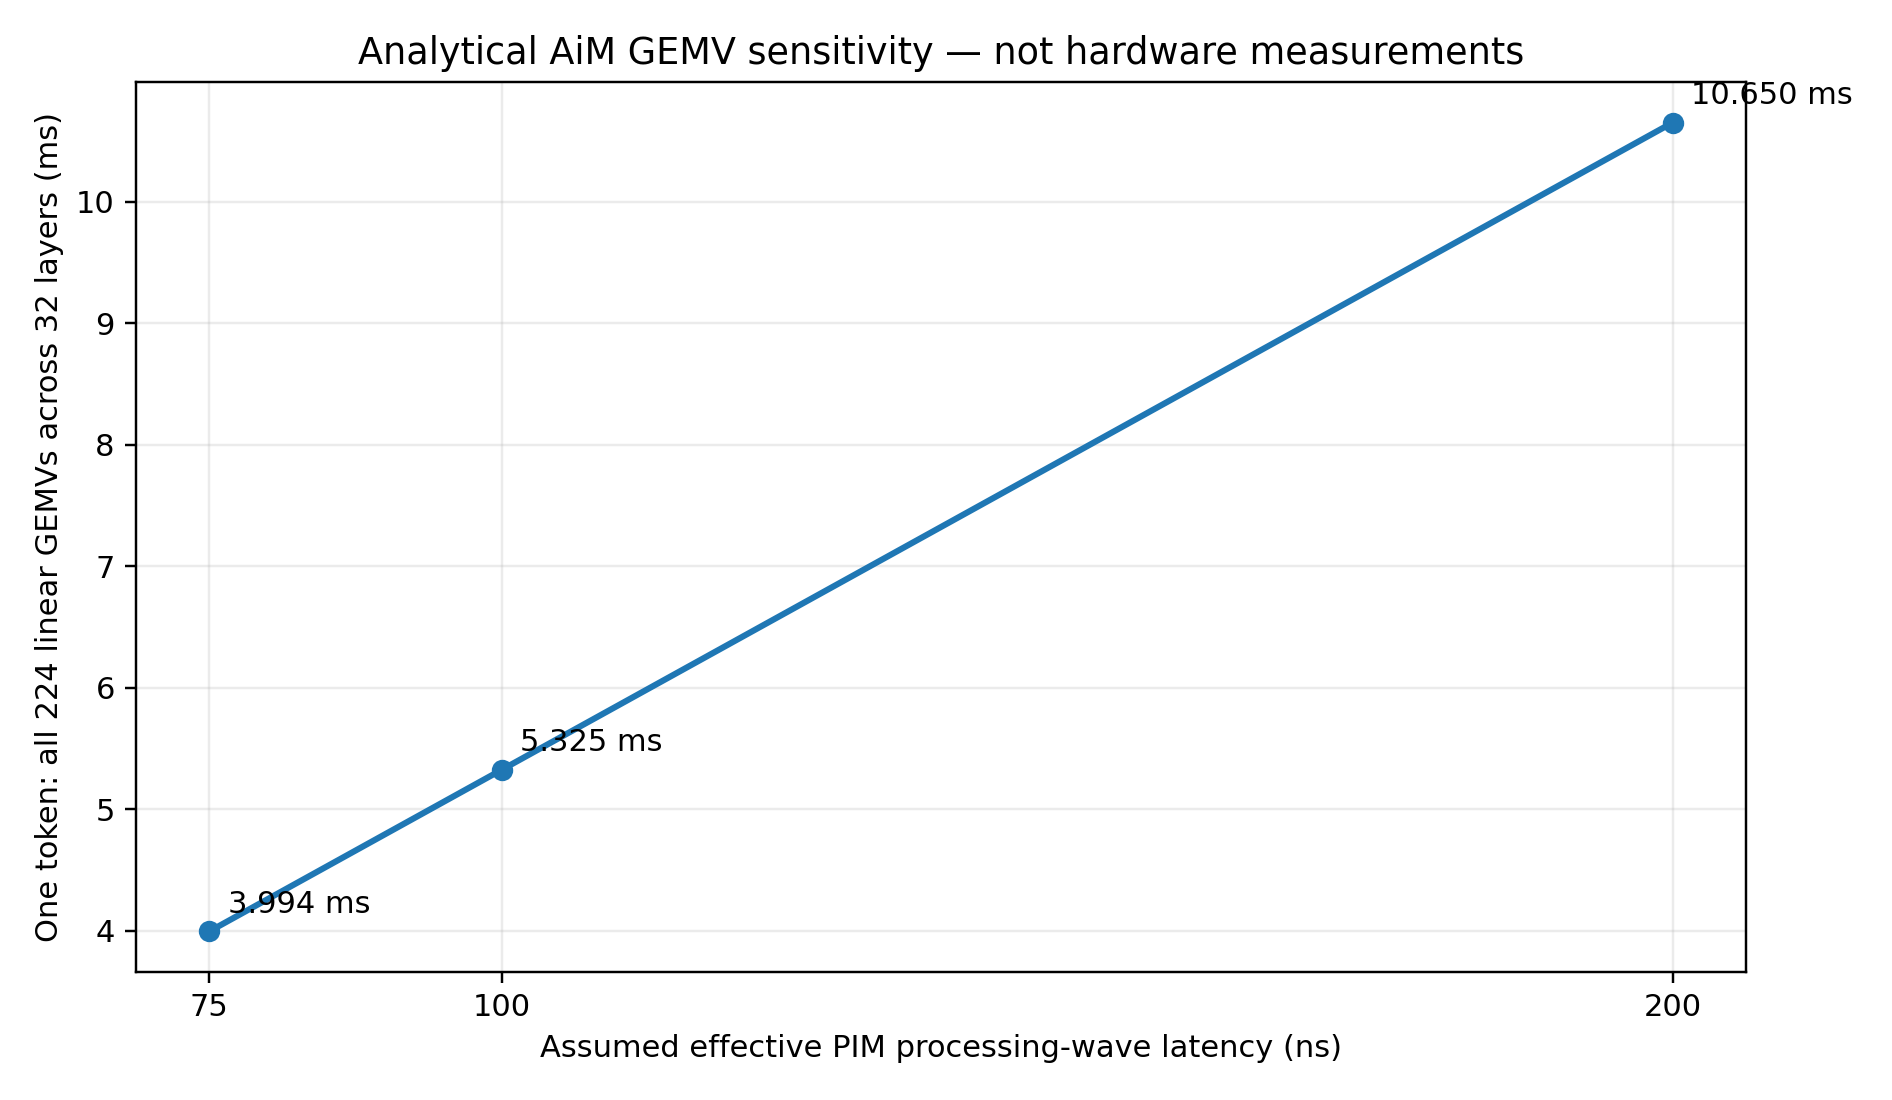
\includegraphics[width=\columnwidth]{pim_gemv_per_token.png}
\caption{Analytical total linear-weight PIM GEMV per token versus
\emph{assumed} effective wave latency (75/100/200 ns); no PIM
hardware measurements are claimed.}
\label{fig:pimwave}
\end{figure}

\section{Original Extension: Batch-Aware Decode Dispatch}
\subsection{Problem and scope}
FACIL's original single-query focus makes PIM-favorable GEMV the
natural decode reference, while its already-established short-prefill
policy considers SoC/PIM execution selection~\cite{facil}. Our
extension studies a distinct workload: \emph{batched decode}, where
$B$ independent sequences supply $B$ token vectors at each decode step.
Their linear projections can be evaluated as SoC GEMM; a simple AiM-style
PIM model instead executes $B$ GEMVs. We select \emph{one engine for the
entire decode step}, not an independent engine per matrix. This is an
analytic policy study, not a claim to invent batched inference or to
implement GPU/PIM instruction scheduling.

\subsection{Reproducible decision model}
For 32 blocks with 224 FP16 linear projections, we use the same four
shapes, multiplicities and peak parameters as the prefill model. For
batch width $B$ and hypothetical SoC efficiency $\eta$,
\begin{align}
C_i(B) &= \frac{2M_iK_iB}{42.5\times10^{12}}, \\[-1pt]
D_i(B) &= \frac{2M_iK_i+2B(M_i+K_i)}{204.8\times10^9}, \\[-1pt]
T_{\rm SoC}(B,\eta) &= \frac{10^3}{\eta}
 \sum_{i=1}^{4}32c_i\max(C_i,D_i),
\label{eq:batchsoc}
\end{align}
where times are in ms, $c_i$ is the per-block projection count,
and 42.5 TFLOP/s and 204.8 GB/s are assumed peak quantities, not
measured batched GEMM performance. The PIM sensitivity model is
\begin{equation}
T_{\rm PIM}(B;T_1,\rho)=T_1[1+(B-1)(1-\rho)],
\label{eq:batchpim}
\end{equation}
with $T_1\in\{5.3248,20\}$ ms. The former uses the
\emph{assumed} 100-ns/wave model (53,248 total projection
waves); the latter is an \emph{illustrative paper-informed scenario},
\emph{not} a paper-measured linear-layer PIM time. Our primary
$\rho=0$ assumption gives linear batch scaling. Positive $\rho$ is a
hypothetical future PIM reuse capability, not established for AiM.
The no-transition-cost policy chooses
$\min(T_{\rm PIM},T_{\rm SoC})$ at each decode step;\ the
original FACIL hardware does not provide a measured transition cost.

\begin{figure*}[t]
\centering
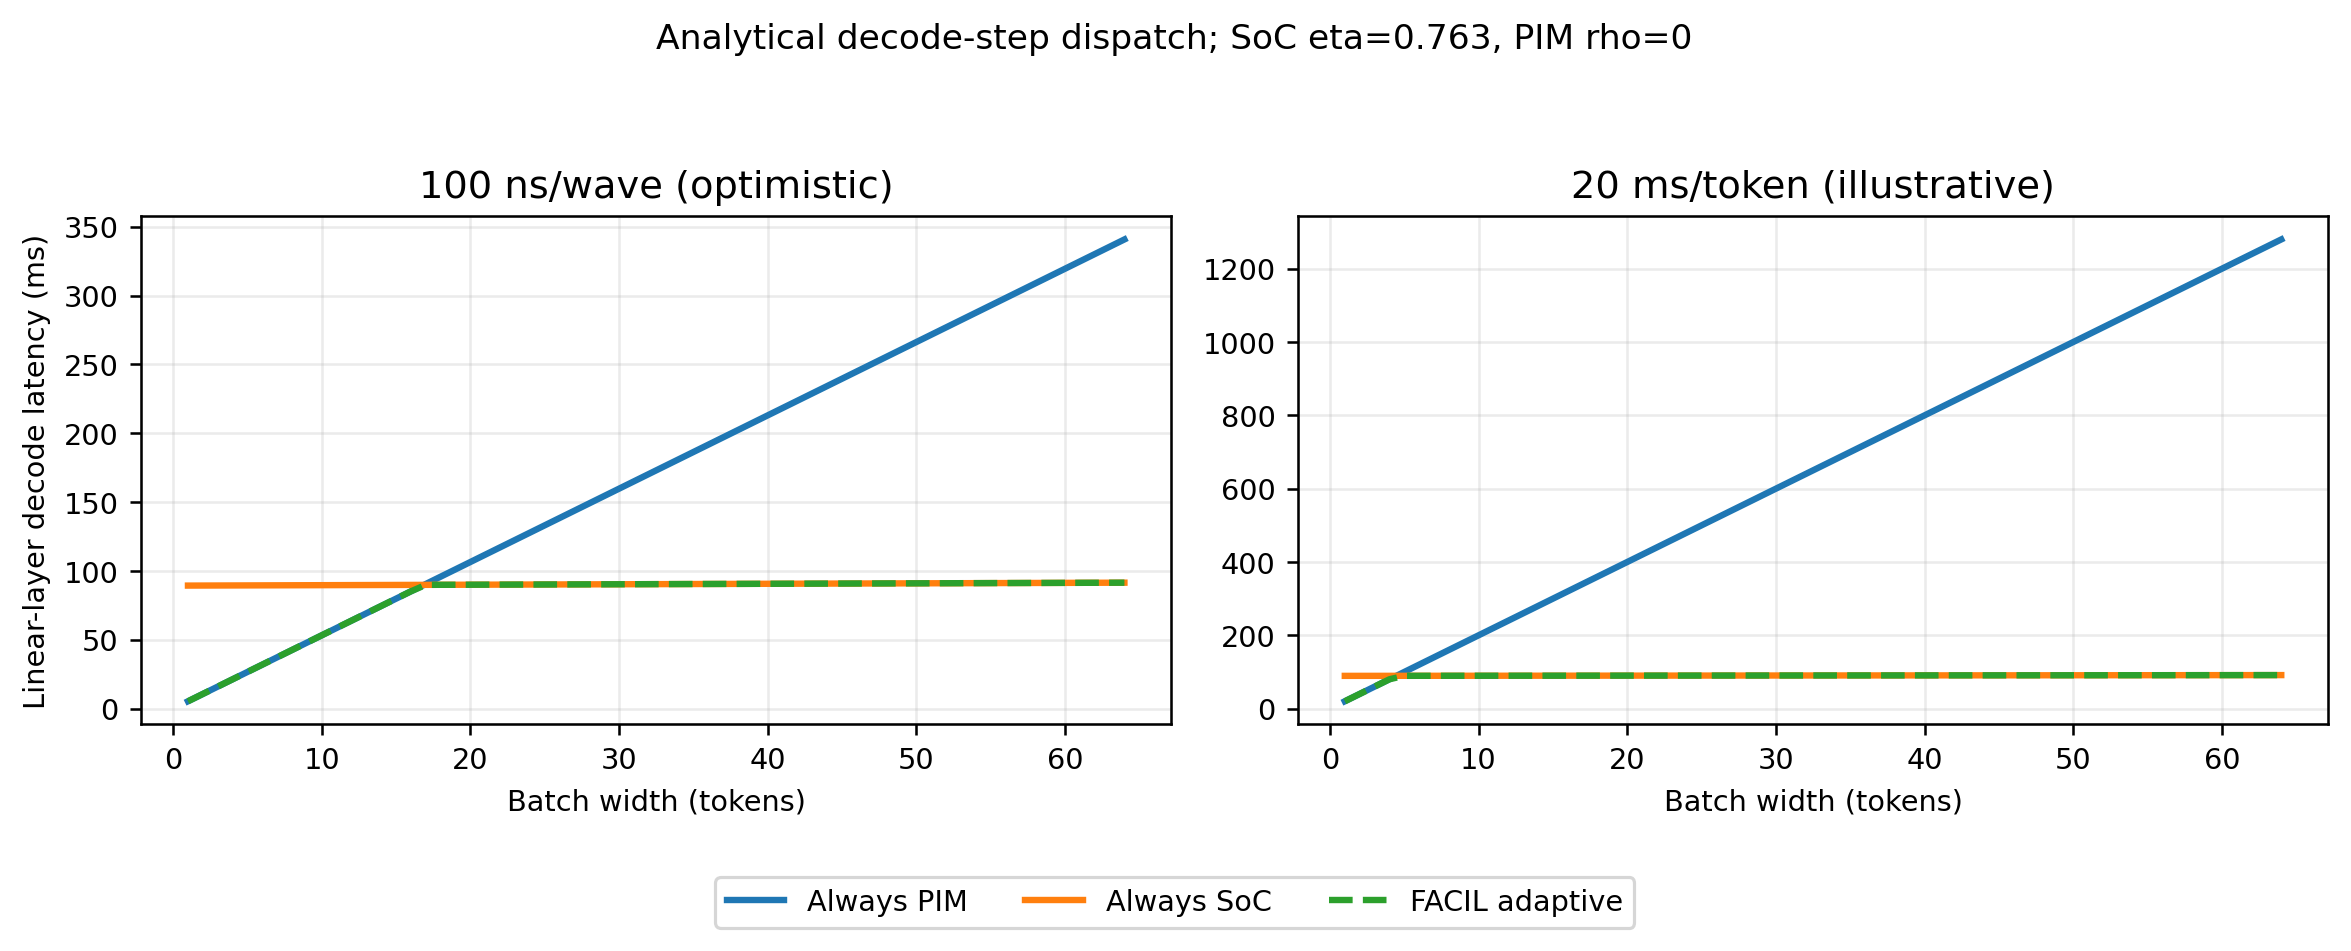
\includegraphics[width=.92\textwidth]{batch_dispatch_two_scenarios.png}
\caption{Linear-projection decode-step latency under two \emph{analytical}
PIM timing scenarios ($\eta=0.763,\rho=0$). The 0.763 value is an assumed
GEMM efficiency sensitivity motivated by the paper's measured GEMV memory
utilization; it is \emph{not} measured GEMM efficiency. Attention, KV
traffic and real PIM switching are excluded.}
\label{fig:batchcompare}
\end{figure*}

\subsection{Experiments 1--2: crossover and robustness}
We sweep $B=1\ldots64$, $\eta\in\{0.30,0.50,0.763,1.00\}$ and
$\rho\in\{0,0.25,0.5\}$. For $\rho=0$ and $\eta=0.763$, the first SoC-favorable
batches are $B=17$ (5.3248-ms scenario) and $B=5$ (20-ms scenario);
for $\eta=0.5$ they are $26$ and $7$. Across the stated tested parameter
combinations, one optimistic low-efficiency, reuse-positive case has no
SoC crossover by $B=64$. These are model breakpoints, not measured
GPU/PIM crossover values.
\begin{figure}[t]
\centering
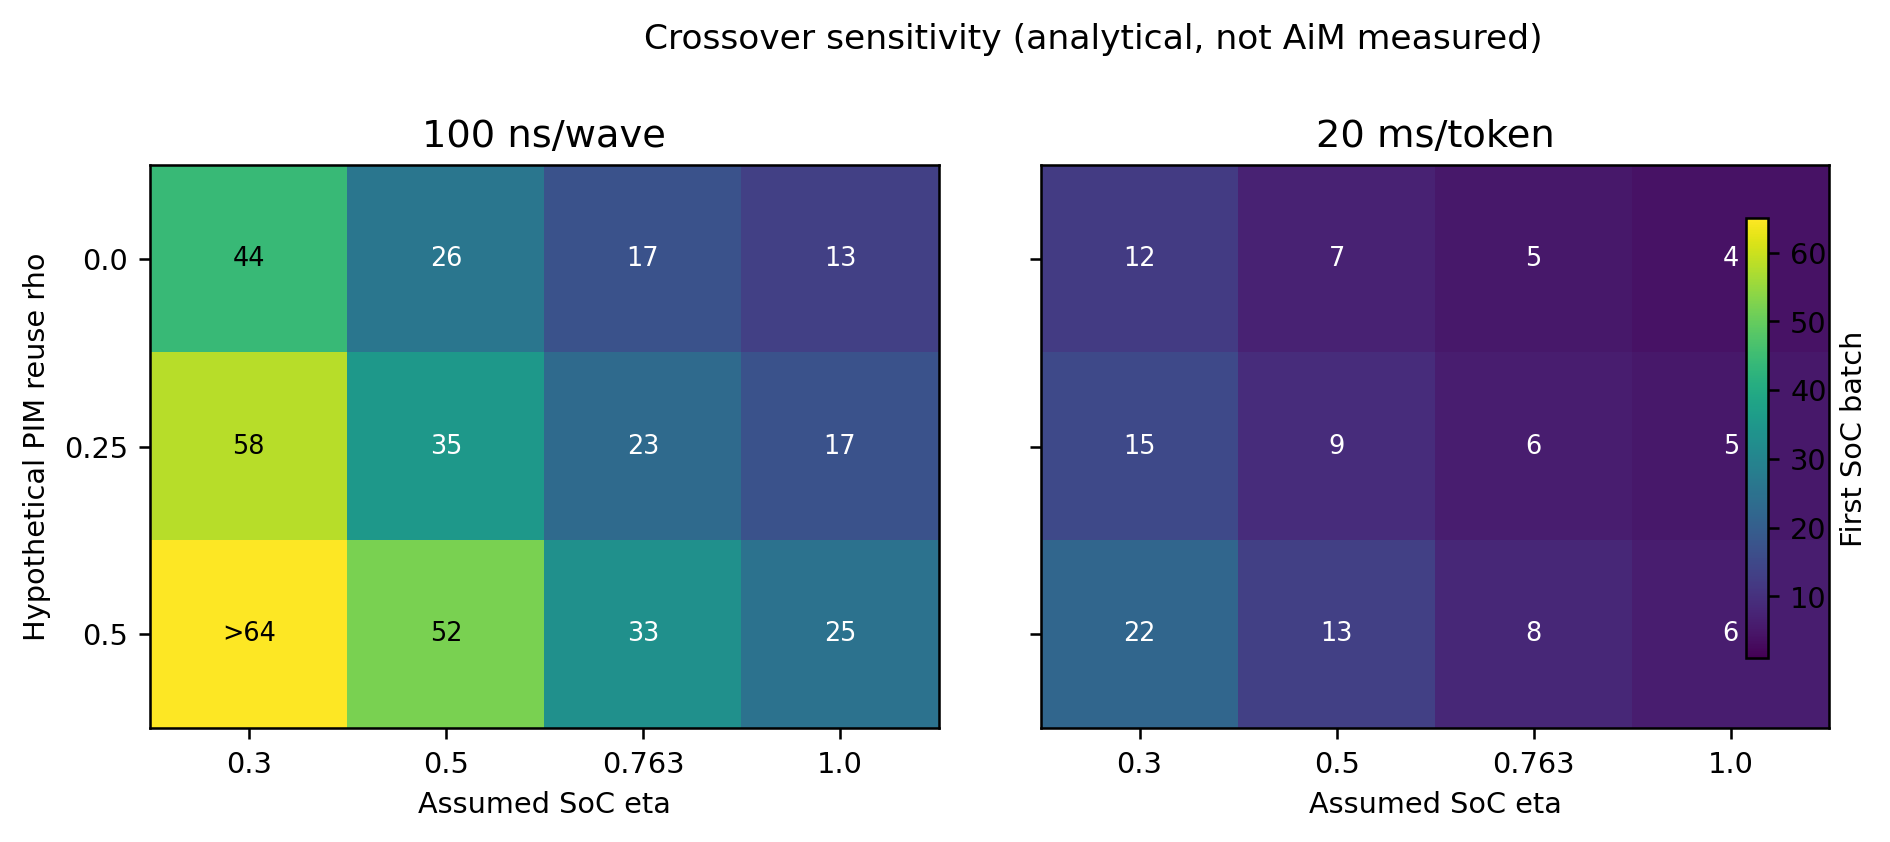
\includegraphics[width=\columnwidth]{batch_crossover_heatmaps.png}
\caption{First SoC-favorable batch versus $\eta$ and hypothetical
PIM reuse $\rho$. A $>64$ cell denotes no crossover within the
sweep, not absence of a crossover at every batch size.}
\label{fig:batchcrossover}
\end{figure}

\subsection{Experiments 3--4: changing batches, memory, transitions}
We evaluate rising $(1,4,16,32,64)$, falling and oscillating
$(1,32,4,64,8,48,2,64)$ sequences. Four execution references are
kept distinct: (i) always-PIM; (ii) all-SoC; (iii) two simultaneous
weight copies, enabling ideal minimum-latency dispatch without
re-layout but doubling linear-weight storage from 13.959 to 27.917
GB; and (iv) the paper-style on-demand re-layout strategy, with a
full modeled conversion for each SoC pass. The latter is evaluated at
447.284 ms (our serialized DRAM-only full-model stage sum) and a
\emph{rough illustrative} 200-ms alternative; the latter is not a
controlled replica of the paper's measured re-layout time. FACIL
provides one-copy re-layout-free access for the adaptive choice,
although runtime transition cost remains unknown. Temporary
conversion buffers and metadata memory are excluded from the
weight-copy-only comparison.

For unmeasured uniform switch overhead $h$, an \emph{offline}
dynamic program finds the best whole-step SoC/PIM sequence when all
future batches are known. Its ideal value is a lower bound on any
online dispatch time. We also evaluate a causal hysteresis heuristic
which switches when the current step's expected saving exceeds $h$.
Rather than assume a specific $h$, we report
\begin{equation}
 h_{\max}=\max_{\pi:\,N_\pi>0,\,T_\pi<T_{\rm static}}
 \frac{T_{\rm static}-T_\pi}{N_\pi},
\label{eq:switchmax}
\end{equation}
where $T_\pi$ is a mixed schedule's zero-overhead total,
$N_\pi$ its transitions and $T_{\rm static}$ the faster of the two
fixed-engine totals. This is the largest uniform transition cost
under which \emph{some offline schedule} still improves on the
best static policy. The first step has a free engine choice, so
initialization cost is excluded.
\begin{table}[t]
\caption{Offline switching-overhead tolerance $h_{\max}$
(ms/transition) under $\eta=0.763$, $\rho=0$.}
\label{tab:batchswitch}
\centering\footnotesize
\begin{tabular}{@{}lrrr@{}}
\toprule
PIM timing & Rising & Falling & Oscillating \\
\midrule
100 ns/wave & 156.868 & 156.868 & 84.037 \\
Illustrative 20 ms/token & 78.824 & 78.824 & 69.362 \\
\bottomrule
\end{tabular}
\end{table}
\begin{figure}[t]
\centering
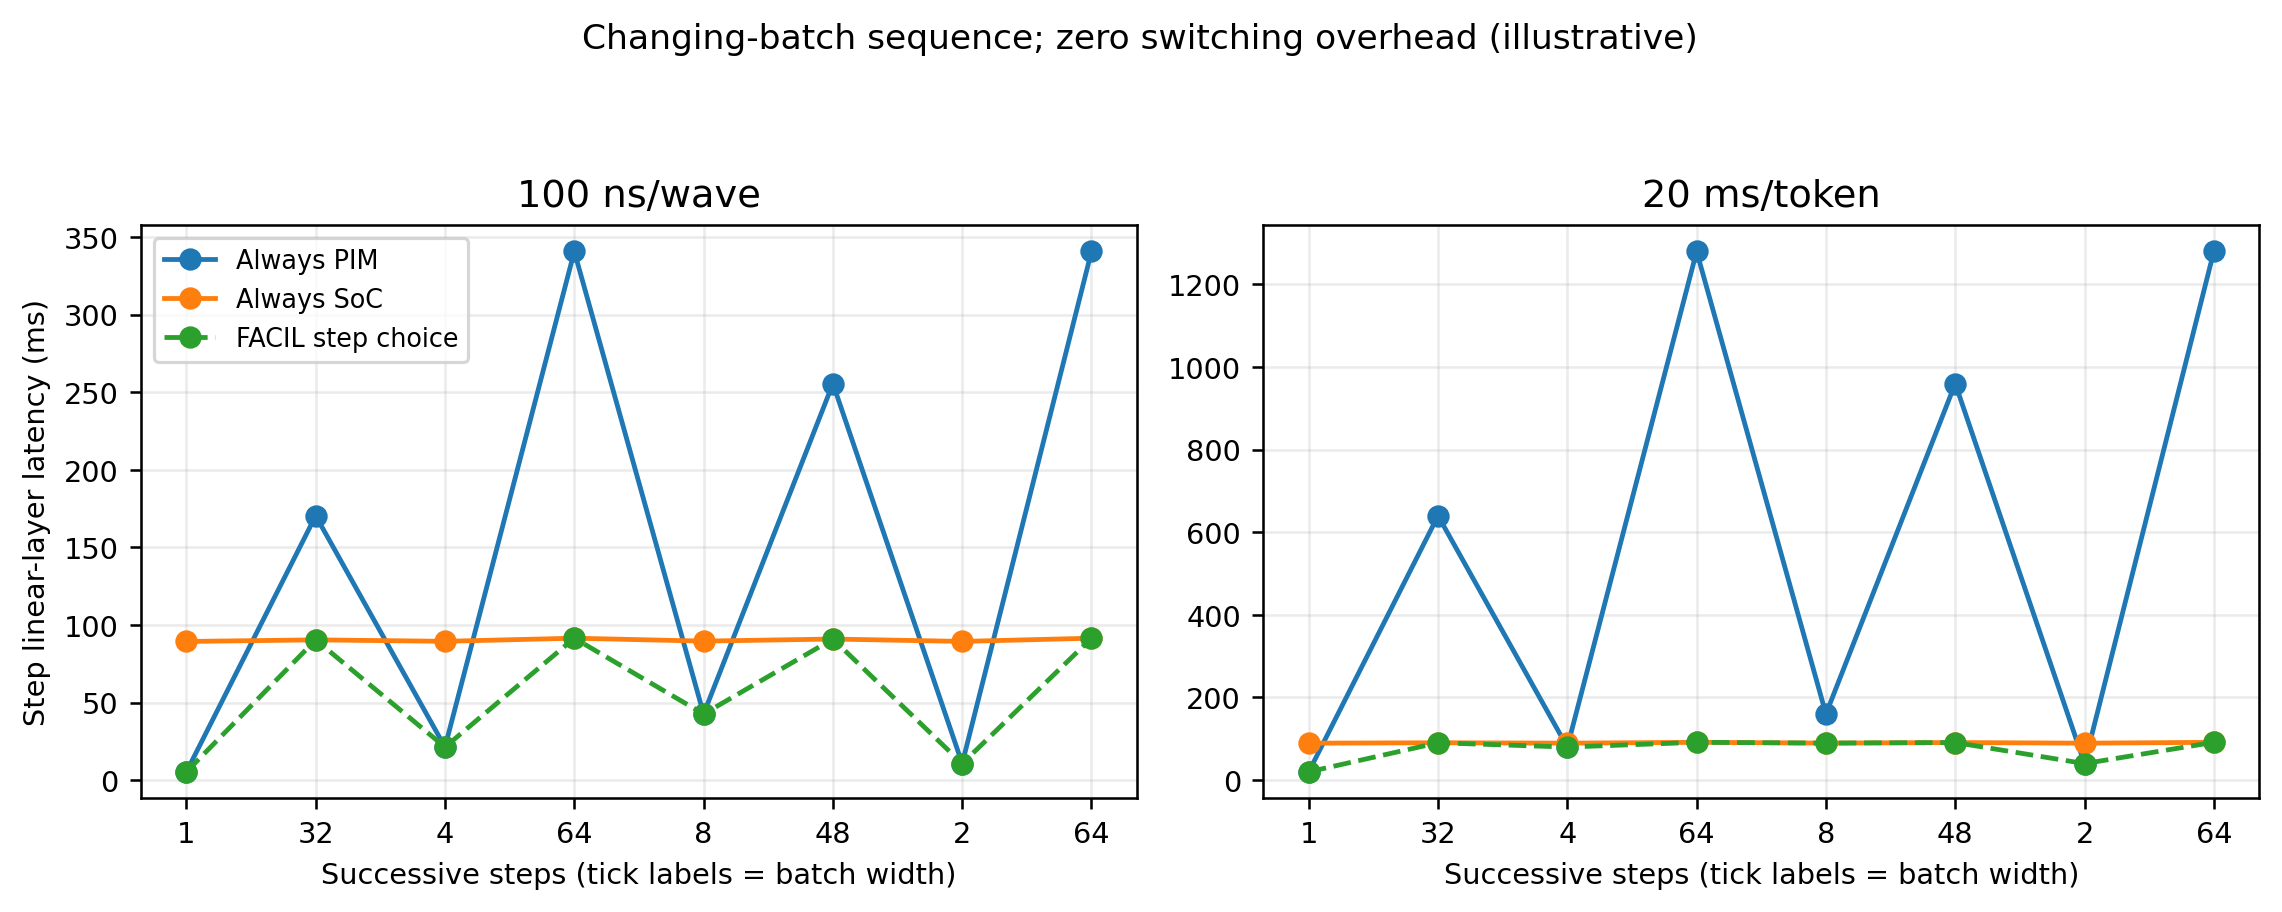
\includegraphics[width=\columnwidth]{batch_dynamic_trace.png}
\caption{Oscillating trace's modeled step costs; zero transition
cost. Under nonzero overhead, decisions change.}
\label{fig:batchtrace}
\end{figure}
\begin{figure}[t]
\centering
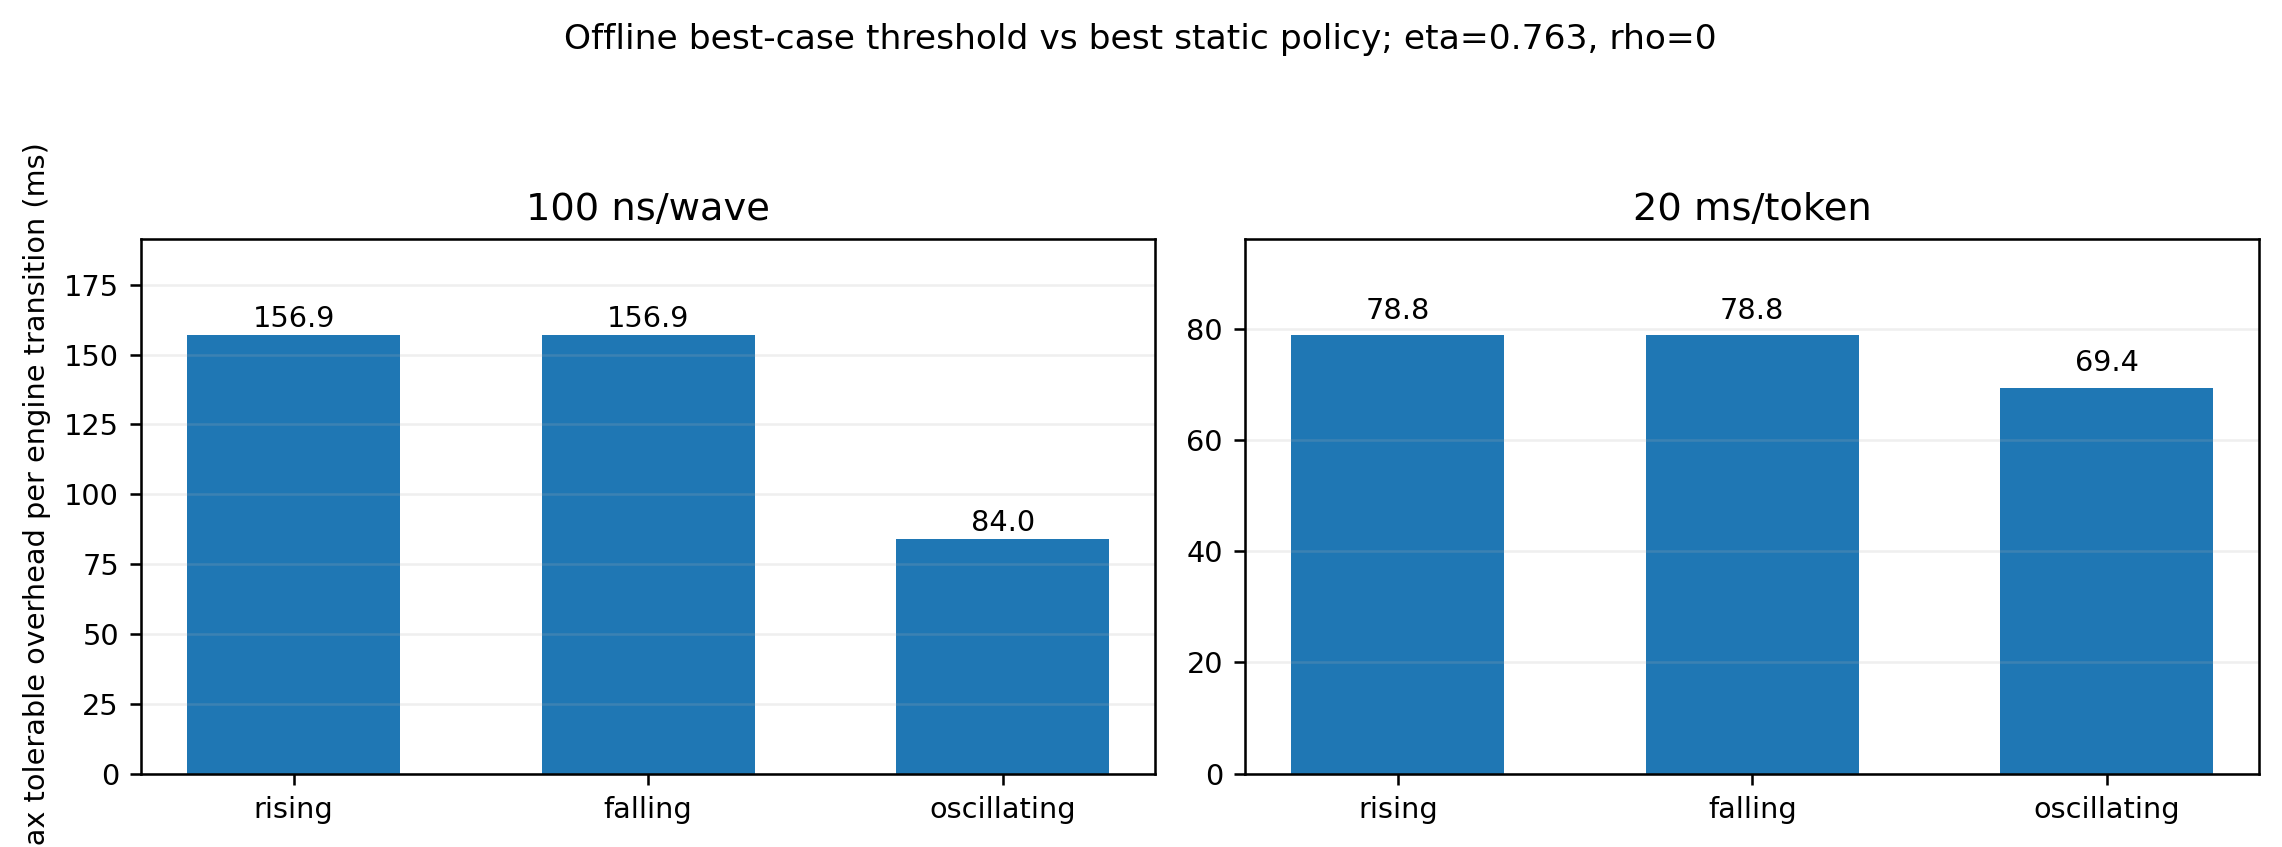
\includegraphics[width=\columnwidth]{batch_switching_hmax.png}
\caption{Maximum tolerable uniform switching cost for an offline
mixed-engine schedule to beat the best static choice, under two
hypothetical PIM scenarios. Not a measured hardware transition cost.}
\label{fig:batchhmax}
\end{figure}

\section{Discussion, Comparison, and Limitations}
\subsection{Modeling limitations and comparison}
\textbf{Timing and protocol fidelity.} The study uses DRAMsim3's LPDDR4
command protocol with LPDDR5-style parameters and synthetic 2-KiB
aggregate bank rows, not validated physical LPDDR5 or calibrated
AiM MAC execution. The original FACIL work uses a different, modified
DRAMsim/real-device methodology~\cite{facil}.

\textbf{Scope of computation.} The SoC model charges one weight read
per projection at ideal Jetson peak bandwidth/compute, but excludes
attention, normalization, nonlinearities, embedding/output layers,
kernel launch, caches, and overlapping execution. The baseline copy
runs two serialized DRAM stages and omits CPU permutation; it is not a
measured end-to-end copy or TTFT.

\textbf{Mapping penalty extrapolation.} Native DRAMsim3 read traces
are sequential logical access proxies. Their FACIL-versus-conventional
time differences do not directly establish changes to real GPU GEMM
kernels; neither a zero penalty nor the $308.964$-ms penalty is a
measured SoC GEMM result. Both are presented only as ideal and
sensitivity scenarios, avoiding double counting of total reads.

\textbf{PIM assumptions.} All 75/100/200-ns wave costs are hypothetical,
with no PIM instruction timing, input broadcast, reduction, or scheduler
calibration. The optional PIM short-prefill model is consequently
optimistic and illustrative rather than an independently measured
speedup.

\textbf{Reference-paper comparison.} FACIL's published Fig.~13 reports
$2.89\times$ geometric-mean Jetson TTFT speedup; its Table~III
reports up to 2.1\% Jetson GEMM slowdown on the PIM layout. Its
real-world-dataset results (Fig.~15) report $2.37\times$ and
$2.63\times$ TTFT speedups after optional dynamic execution
selection~\cite{facil}. The modeled ideal speedups ($7.26$--$7.54\times$)
and extrapolated read-penalty speedups ($1.364$--$1.367\times$) are
\emph{not} apples-to-apples reproductions: they use a restricted
linear-only workload, ideal roofline, synthetic DRAM timings, and a
different penalty assumption. The no-extra-copy mechanism is reproduced
and model trends are studied, not the original percentages.

\textbf{New decode policy limitations.} Batch-width-aware selection
is implemented as an analytical step-level policy, not an SoC/PIM
runtime. The optimistically modeled 5.325-ms PIM time and illustrative
20-ms time are unmeasured; $\rho>0$ is hypothetical and $\eta=0.763$
is borrowed as a \emph{sensitivity setting} from a different GEMV
metric. Attention, KV-cache access, GPU kernel launches, time-varying
memory contention, real PIM broadcast/reduction, queues and model
capacity are excluded. Consequently our modeled decode linear-layer
latencies cannot be labeled end-to-end TTLT or hardware speedup.
Duplication can match zero-overhead FACIL dispatch latency but
requires an additional 13.959 GB of linear weights in the model.

\subsection{Exploratory FFN-down row padding}
A row-stride alignment experiment produced a negative result:
a 28-KiB to 32-KiB FFN-down row-stride change eliminates 48
huge-page crossings and makes all rows use two PUs. However, it
raises footprint from 112 to 128 MiB (+14.3\%), requires
nondefault SoC leading dimension and increases sampled native
READ completion from 127.411 to 141.907 $\mu$s. Structural
regularity alone did not yield measured speedup in this test.

\section{Reproducibility}
The experiments use a fixed four-channel, two-rank DRAMsim3
configuration and the FP16 matrix shapes in Table~\ref{tab:layers}.
Mapping and placement are verified by \texttt{facil\_mapper.py}
and native C++ decoder tests. Trace construction and DRAM traffic
are reproducible with
\texttt{generate\_verified\_baseline\_traces\_2k.py},
\texttt{measure\_relayout.py} and
\texttt{facil\_step3\_ffn\_reads.py}. The analytical SoC/PIM
models use \texttt{llama3\_soc\_gemm\_roofline.py} and
\texttt{facil\_pim\_gemv\_analytical.py}; batch-width sweeps and
transition policies use \texttt{facil\_batch\_exp12.py} and
\texttt{facil\_batch\_exp34.py}. The bandwidth diagnostic uses
\texttt{facil\_batch\_exp5.py}.

The relevant configuration, trace manifests, transaction counts,
analytical parameter values and model results are retained to
permit replication. The model does not simulate OS modifications,
PIM arithmetic or end-to-end inference; these require additional
hardware-level evaluation.

\section{Conclusion}
The reduced-scope FACIL reproduction confirms MapID placement and
native DRAMsim3 routing on four FP16 Llama3 projection classes,
and reports an explicitly qualified 447.284-ms serialized baseline
copy-stage sum. The prefill first-token models remain theoretical
proxies, not device TTFT measurements. Our independently implemented
batch-width-aware decode-step selection model identifies SoC/PIM
crossovers under two declared PIM timing scenarios and evaluates
changing batches, the memory cost of an ideal duplication baseline,
and the offline tolerance for unmeasured switching overhead. The
analytic model can match ideal two-copy dispatch latency with a
single weight copy under FACIL, but proves no real-device speedup.
An access-order DRAMsim3 sample reports a 3.05$\times$ improvement
in completed-read throughput for a sequential trace, while the FFN-down padding experiment shows a negative result.
These results establish an implemented and evaluated student-scale
policy extension, with explicit performance and fidelity limits.

\section*{Team Contributions (To Be Completed)}
\noindent\textit{The following details will be completed by both authors
before submission.}\par\smallskip
\noindent\textbf{Member 1:} \textit{[Name and individual responsibilities]}\par
\noindent\textbf{Member 2:} \textit{[Name and individual responsibilities]}\par
\noindent\textbf{Joint contributions:} \textit{[To be completed]}\par

\balance
\begin{thebibliography}{9}
\bibitem{facil} S.~H. Seo, J. Kim, D. Lee, S. Yoo, S. Moon,
Y. Park, and J.~W. Lee, ``FACIL: Flexible DRAM Address Mapping for
SoC--PIM Cooperative On-device LLM Inference,'' in \emph{Proc.
IEEE International Symposium on High-Performance Computer
Architecture (HPCA)}, 2025, doi:10.1109/HPCA61900.2025.00127.
\bibitem{dramsim3} S. Li, Z. Yang, D. Reddy, A. Srivastava,
and B. Jacob, ``DRAMsim3: A cycle-accurate, thermal-capable DRAM
simulator,'' \emph{IEEE Computer Architecture Letters}, vol. 19,
no. 2, pp. 106--109, 2020, doi:10.1109/LCA.2020.2973991.
\bibitem{dramsim3repo} University of Maryland Memory Systems
Research Group, ``DRAMsim3 source repository,''
\url{https://github.com/umd-memsys/DRAMsim3}.
\end{thebibliography}
\end{document}
